% !TeX root = ../main.tex
\chapter{Matlab仿真实验}
仿真实验分为两部分,Matlab和ROS。Matlab中的模型更接近于理想,而Ros中的模型和控制器更接近于实际。Matlab中基于s-function和simulink的仿真,主要是为了在理论层面验证控制算法的性能。在这一章中,我们将与经典的SO(3)控制和PX4中的四环PID控制(后简称PID)对比,说明HOFA方法的优越性。



\section{实验设计}
我们在Simulink环境下构建了一个综合仿真模型,该模型不仅包含了刚体动力学和电机动态,还通过s-function实现了姿态环和位置环分离的双环控制器设计。这种设计使得后续的数据分析和研究工作能够更为便捷、高效。

\textbf{轨迹设计}

为了能直观地体现性能,我们设计了一个“8”字型轨迹,如图\ref{fig:8}:
$$x_d = \begin{matrix}[5\sin(\frac{t}{2}), & 5\cos(\frac{t}{2})\sin(\frac{t}{2}), &-0.1t]\end{matrix}
\quad
\psi_d=0.01t$$

\begin{figure}[!h]
  \centering
  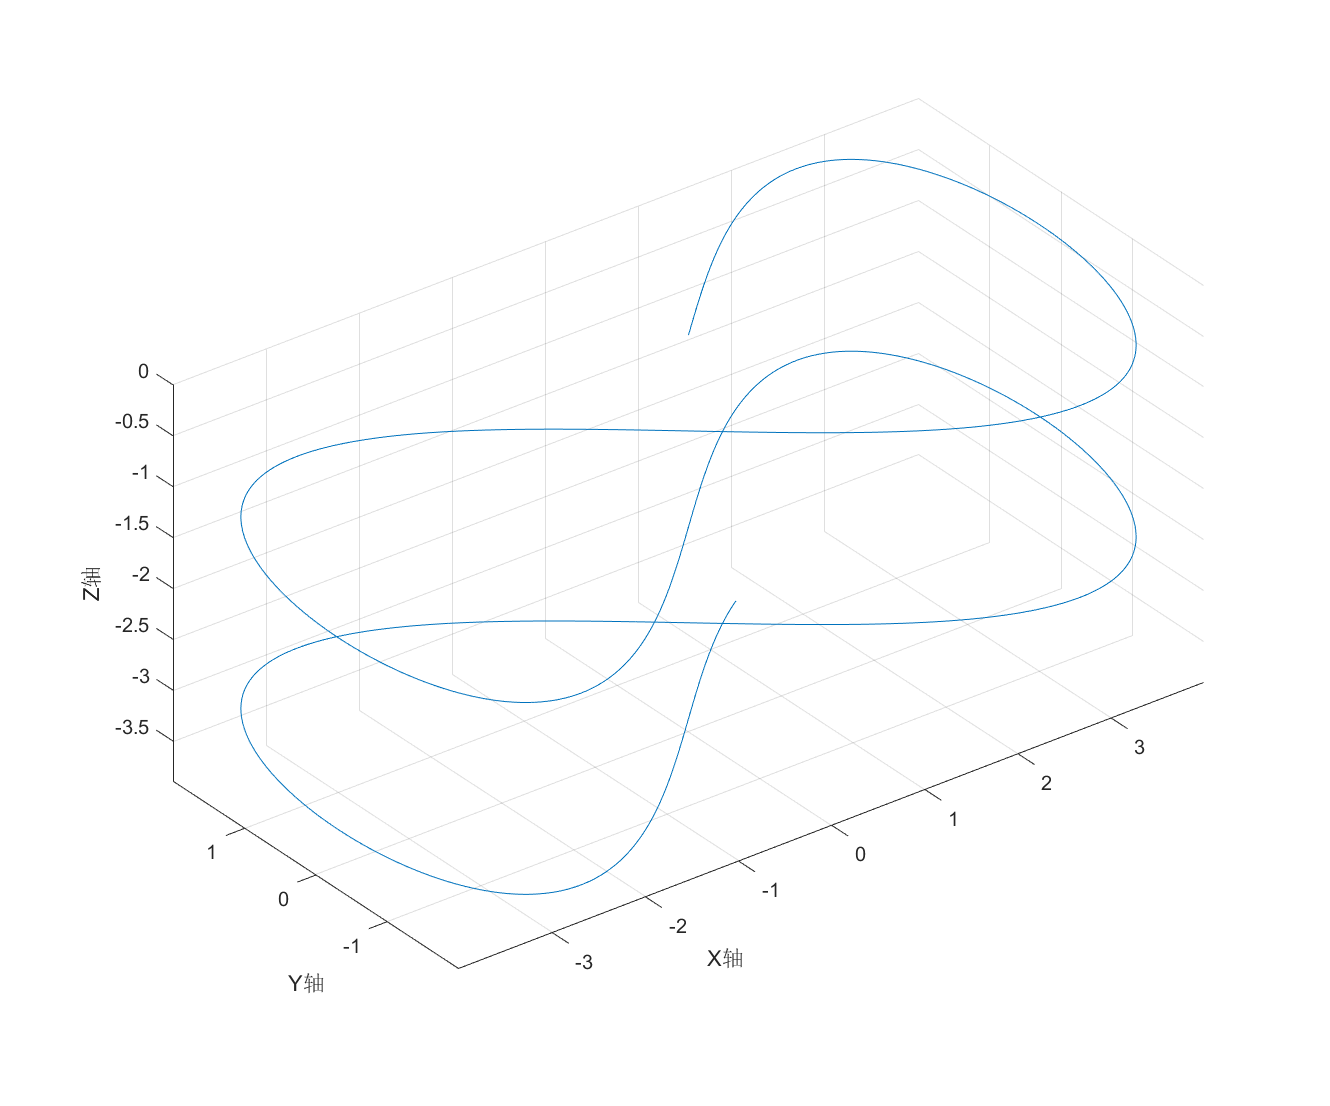
\includegraphics[width=0.5\textwidth]{88.png}
  \caption{高度匀速上升的“8”字型轨迹(北-东-地坐标系下,地面以上Z轴为负数)}
  \label{fig:8}
\end{figure}

为了全面体现控制算法的跟踪性能,我们并没有对轨迹做特殊的平滑处理,轨迹的导数存在间断点使得高阶导数无穷大,这可以考验无人机在现实中的抗扰性能。为了模拟起飞和悬停,第一秒内轨迹保持在原点不动,否则仿真就会等同在空中释放电机无转速的无人机。

\textbf{被控对象}

  无人机的刚体动力学部分由simulink中自带的“6DOF block”解决,避免了$SO(3)$群差分近似后单位化的困难。该模块会对外部输入的力和力矩做出反应,返回所需的速度、位置、姿态、角速度等信息。

  电机部分,转速的动态由一阶惯性环节表示,根据所选电机型号时间常数$\tau=0.01s$。
  姿态控制器和位置控制器分开由两个s-function实现,重力由单独的模块输入到“6DOF block”。
  \begin{figure}[!h]
    \centering
    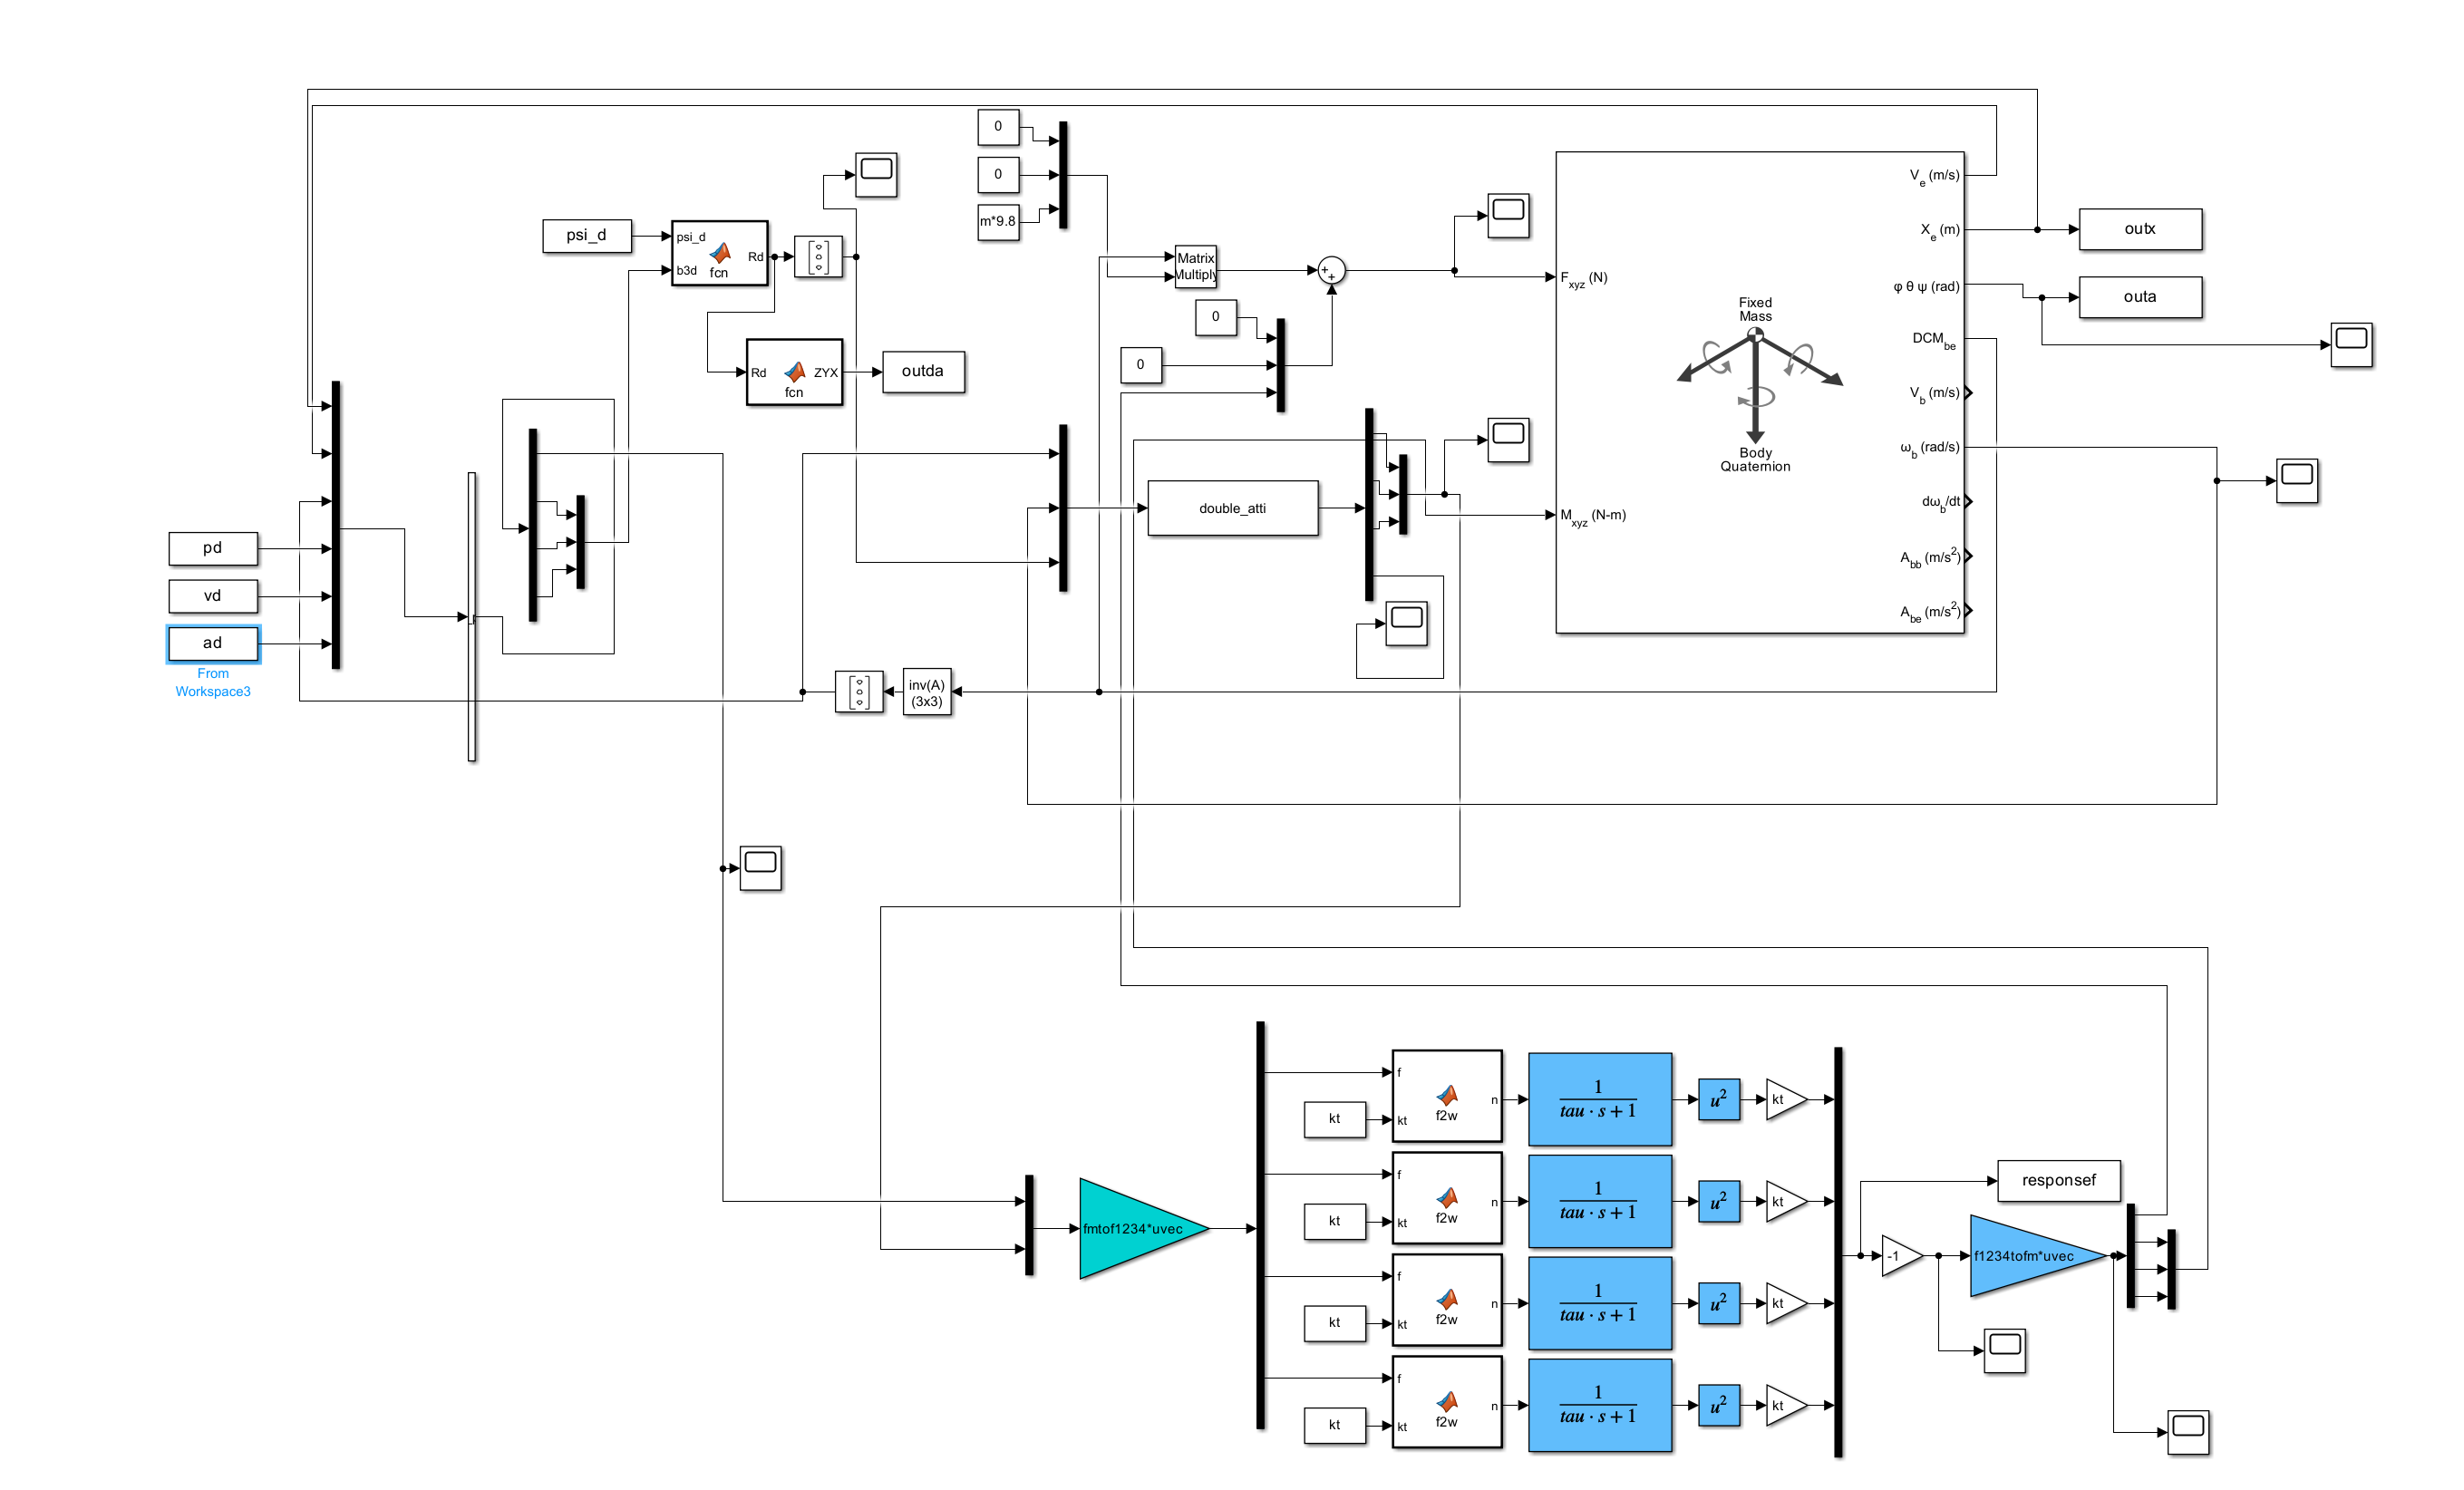
\includegraphics[width=0.9\textwidth]{sim.png}
    \caption{simulink仿真连线图}
    \label{fig:sim}
  \end{figure}

  \textbf{模型参数}

  质量参数由最终实飞的无人机测量得到,详见实机实验一章:
  $$m=0.8771kg \quad d=0.125m \quad J=\begin{bmatrix}
    0.0031   &      0  &       0\\
    0 &   0.0032      &   0\\
    0  &       0   & 0.0045
  \end{bmatrix}kg m^2$$

  电机参数由厂家数据得到:
  $$k_t=2.03\times 10^{-8} \quad 
  \tau=0.01s \quad
  c_{\tau f}=8\times 10^{-3}$$

  选择替补姿态控制律:
  $$k_R=0.881 \quad k_\omega=0.254$$

  位置环和姿态环的LQR权重矩阵分别为:
  $$Q_x=\begin{bmatrix}
    10&0&0&0&0&0\\
    0&10&0&0&0&0\\
    0&0&10&0&0&0\\
    0&0&0&3&0&0\\
    0&0&0&0&3&0\\
    0&0&0&0&0&3\\
  \end{bmatrix}, \quad R_x=\begin{bmatrix}
    0.1 &0 &0\\
    0 &0.1 &0\\
    0 &0 &0.1\\
  \end{bmatrix}$$

  $$Q=\begin{bmatrix}
    100&0&0&0&0&0\\
    0&100&0&0&0&0\\
    0&0&30&0&0&0\\
    0&0&0&0.1&0&0\\
    0&0&0&0&0.1&0\\
    0&0&0&0&0&0.1\\
  \end{bmatrix}, \quad R=\begin{bmatrix}
    0.01 &0 &0\\
    0 &0.01 &0\\
    0 &0 &0.01\\
  \end{bmatrix}$$

  初始位姿:
  $$x(0)=[0,0,0],\quad v(0)=[0,0,0]$$
  $$R(0)=I , \quad \omega(0)=[0,0,0]$$

  \textbf{限幅}

  期望值的传递链路是$x_d \to v_d \to R_d \to \omega_d \to \alpha_d$。在这条链路中,除了$ v_d \to R_d$的传递,其他三次都会带来微分,会放大上一环节的噪声。如果放任冲击信号进入控制器,会对系统造成不良影响,因此需要做相应的限幅。但因为期望拉力最大不过接近水平,所以$R_d$这一环节本身就带有限幅,在Matlab仿真中就不做额外限幅以获得更激进的控制效果,同时也能更好地测试姿态环的鲁棒性。

  \section{实验结果与分析}

  按照上述参数,在Matlab中用0.005s的控制周期分别运行HOFA、PID和SO(3)控制。输入典型的阶跃和斜坡信号对比其控制性能,由于俯仰与滚转对称,仅选择俯仰模态(x轴)进行实验。

  \textbf{单位阶跃输入}

  在$t=1s$时对x轴输入单位阶跃信号,对比x轴位置、速度、角度、角速度和期望扭矩,如图\ref{matlab_阶跃}。由于另外两轴仅受到轻微的耦合影响,且不是研究对象,为精简篇幅,不在此罗列另外两轴的数据。

\begin{figure}[h]
  \centering
  \begin{subfigure}[t]{0.33\textwidth}
    \centering
    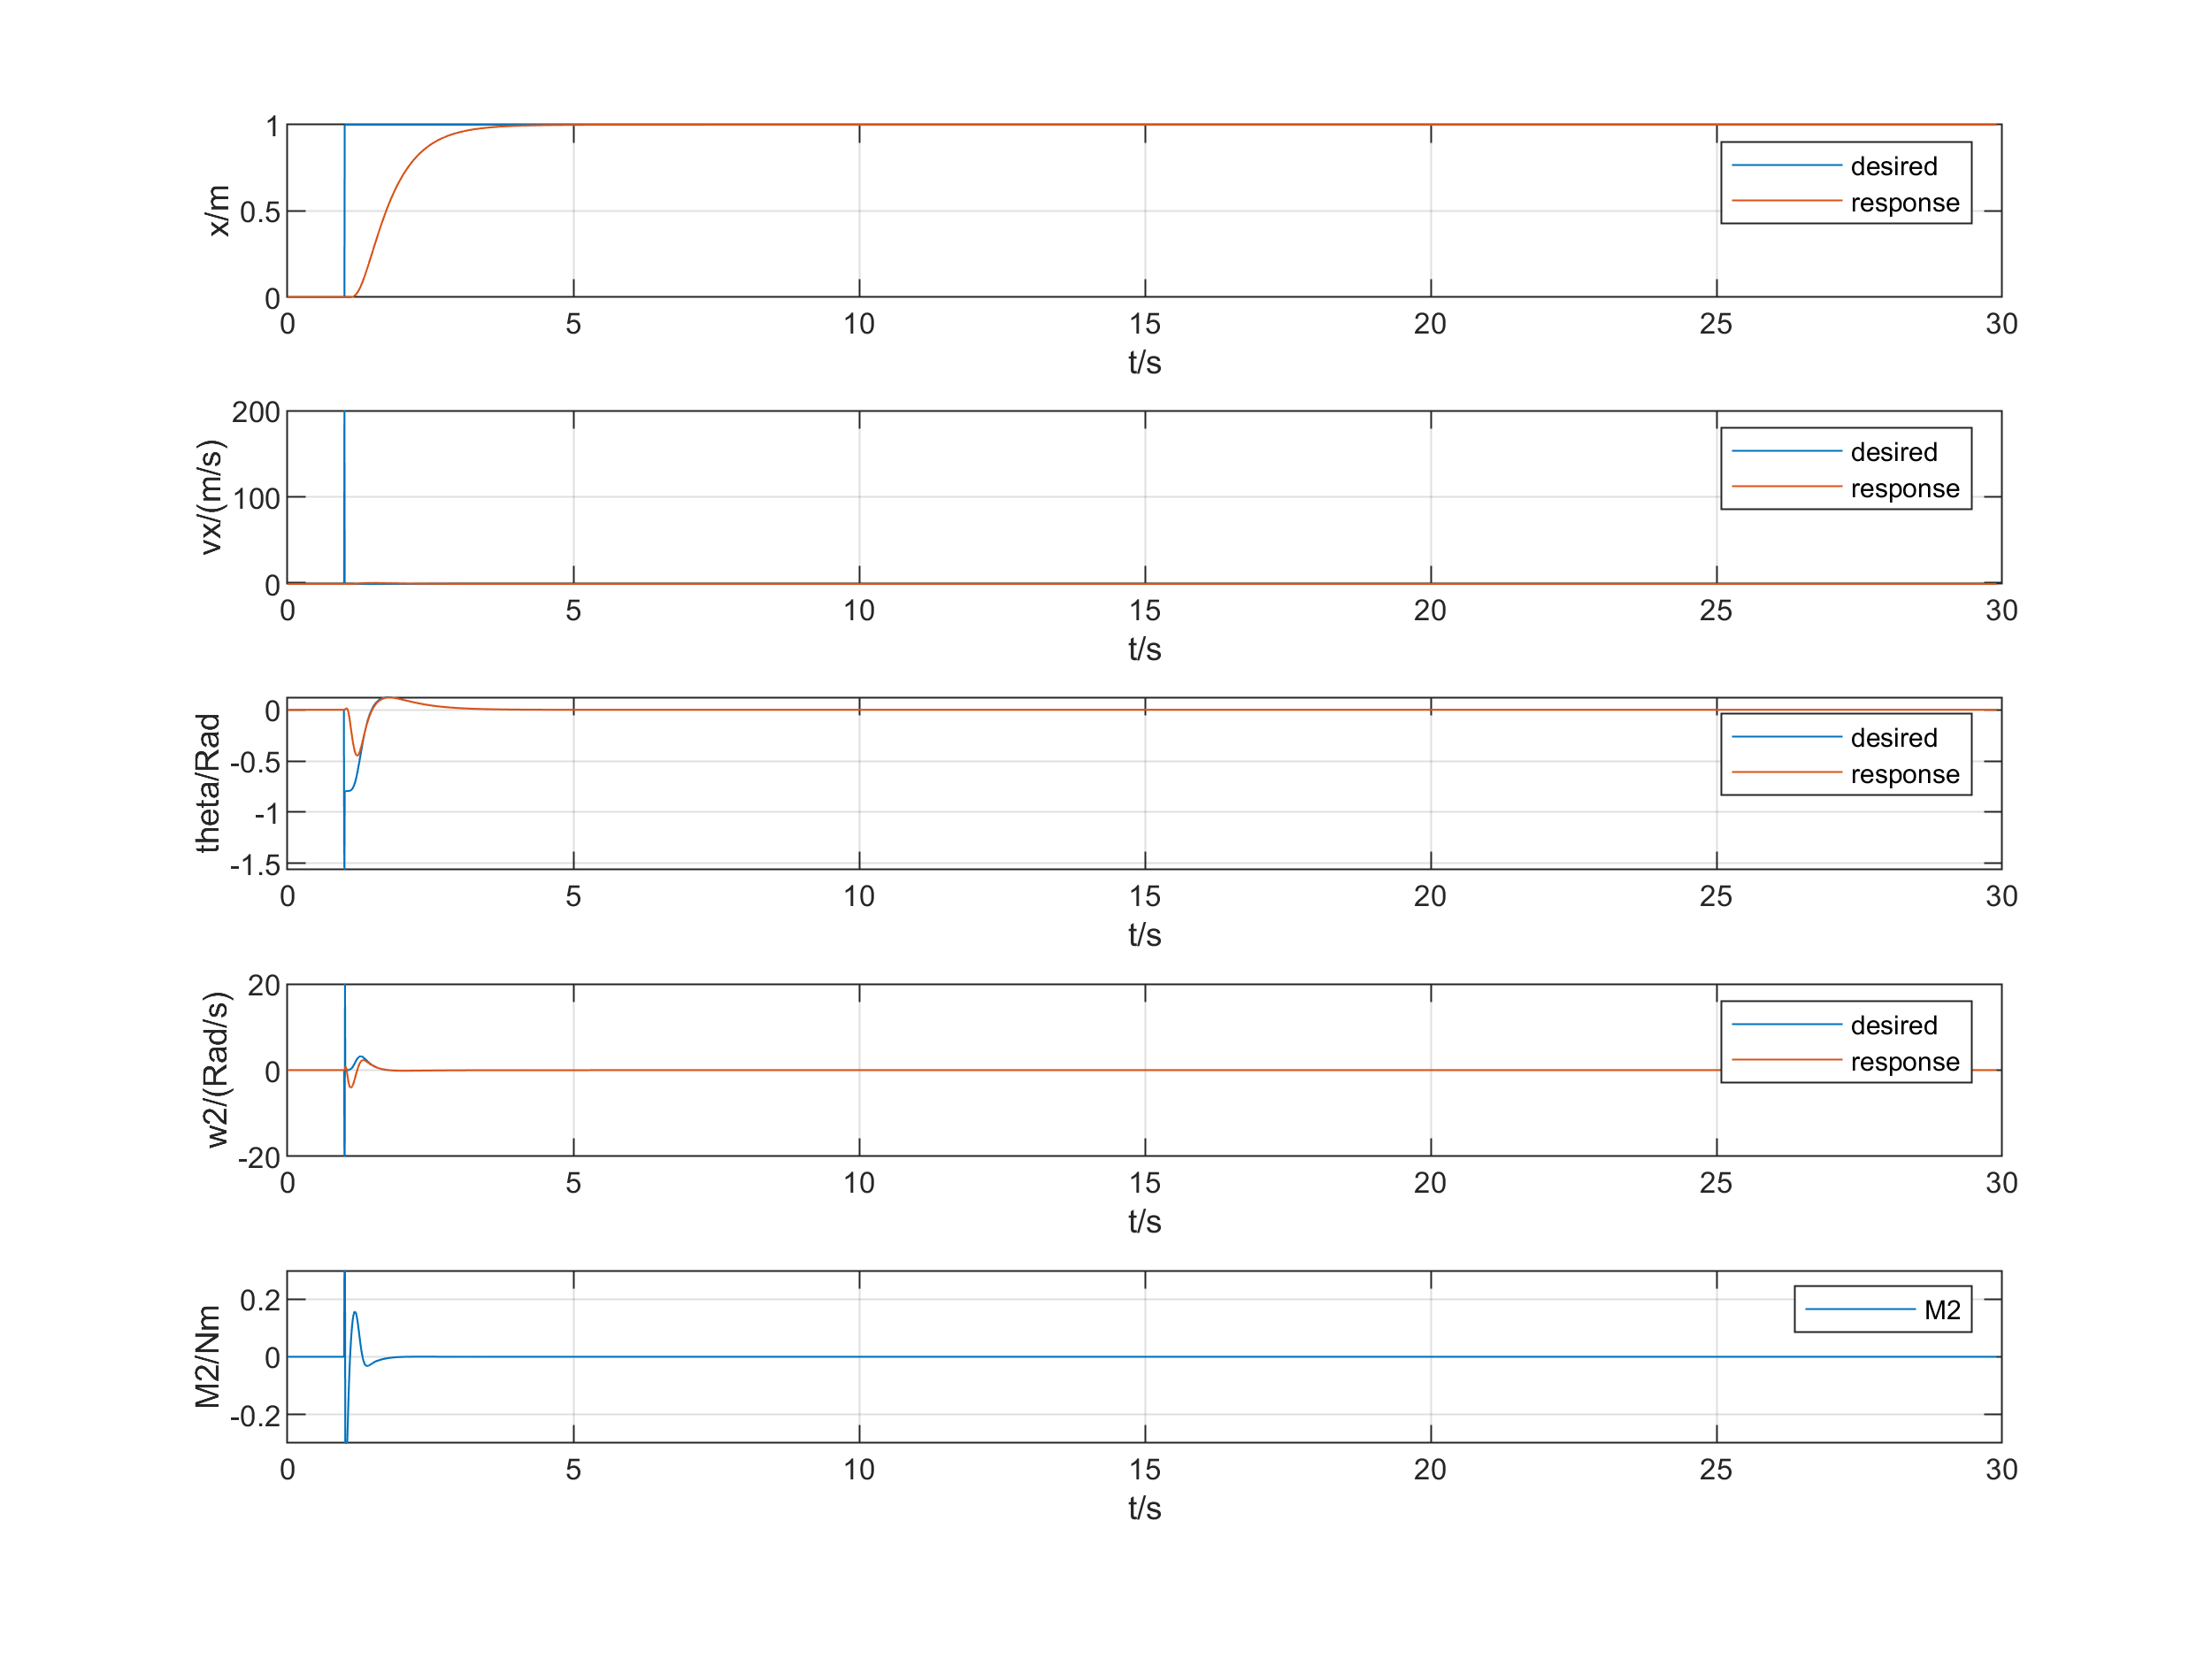
\includegraphics[width=\linewidth]{hofa_1.png}
    \caption{HOFA}
  \end{subfigure}\hfill
  \begin{subfigure}[t]{0.33\textwidth}
    \centering
    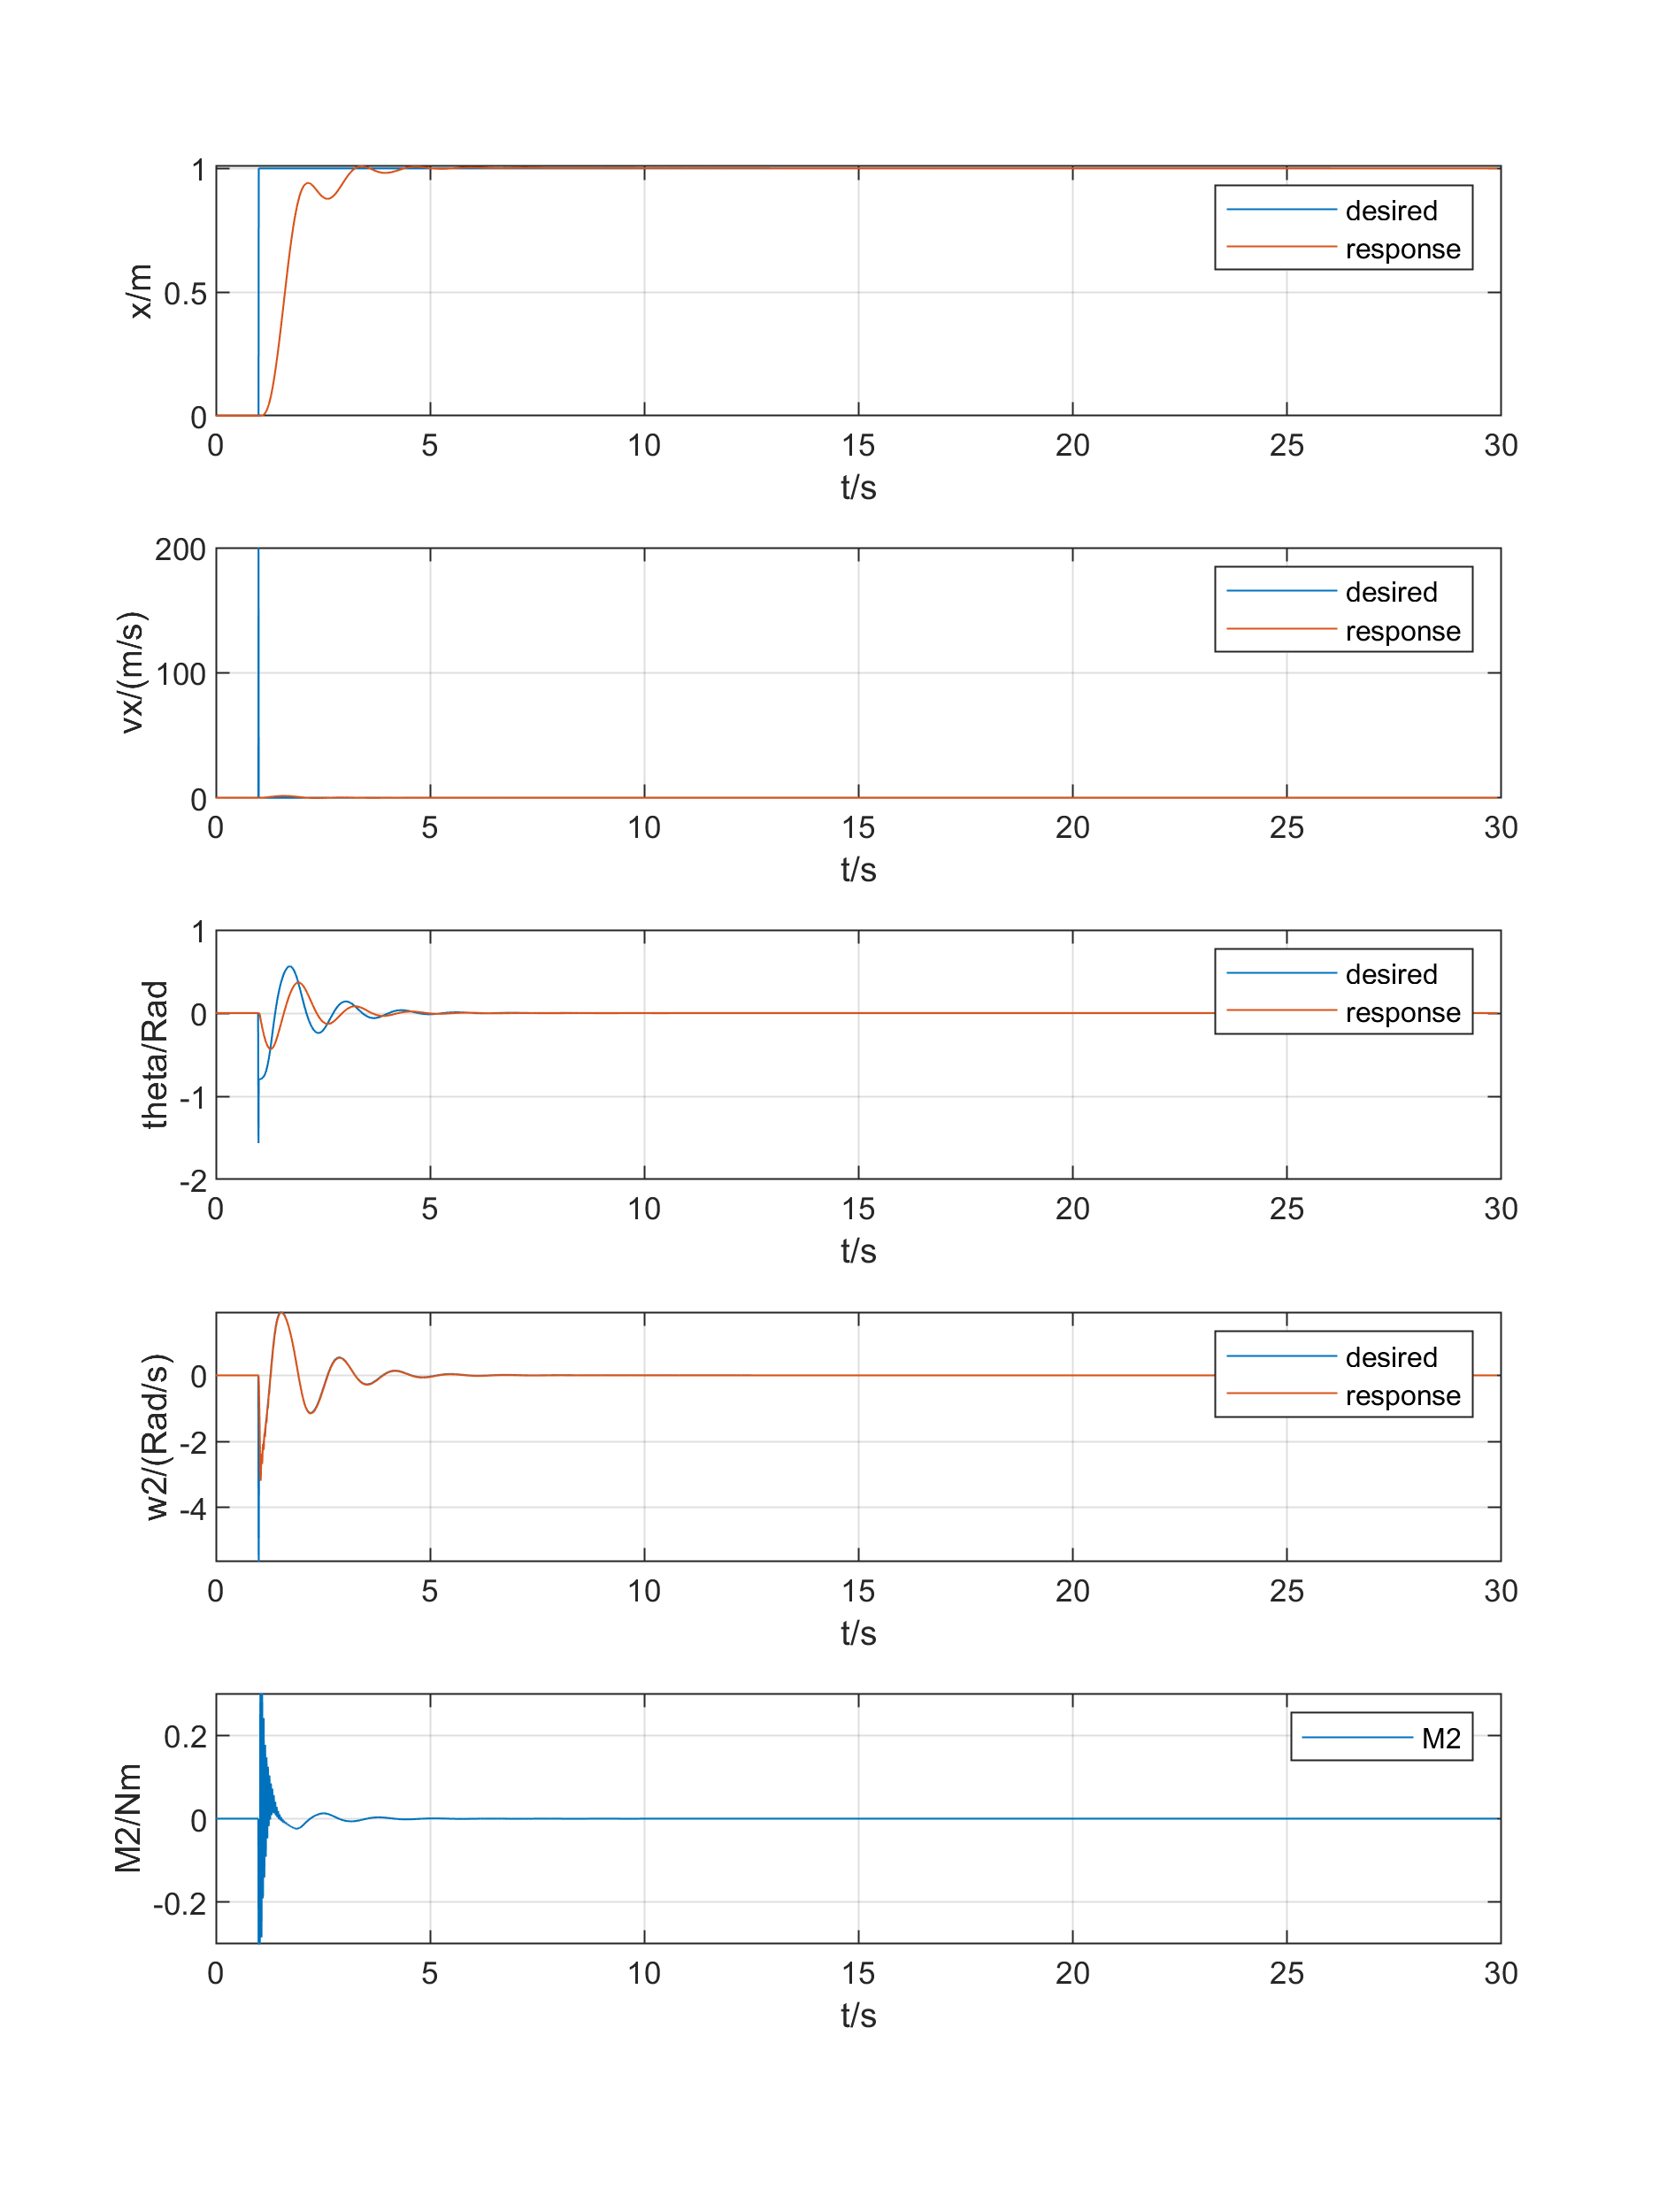
\includegraphics[width=\linewidth]{px4_1.png}
    \caption{PID}
  \end{subfigure}\hfill
  \begin{subfigure}[t]{0.33\textwidth}
    \centering
    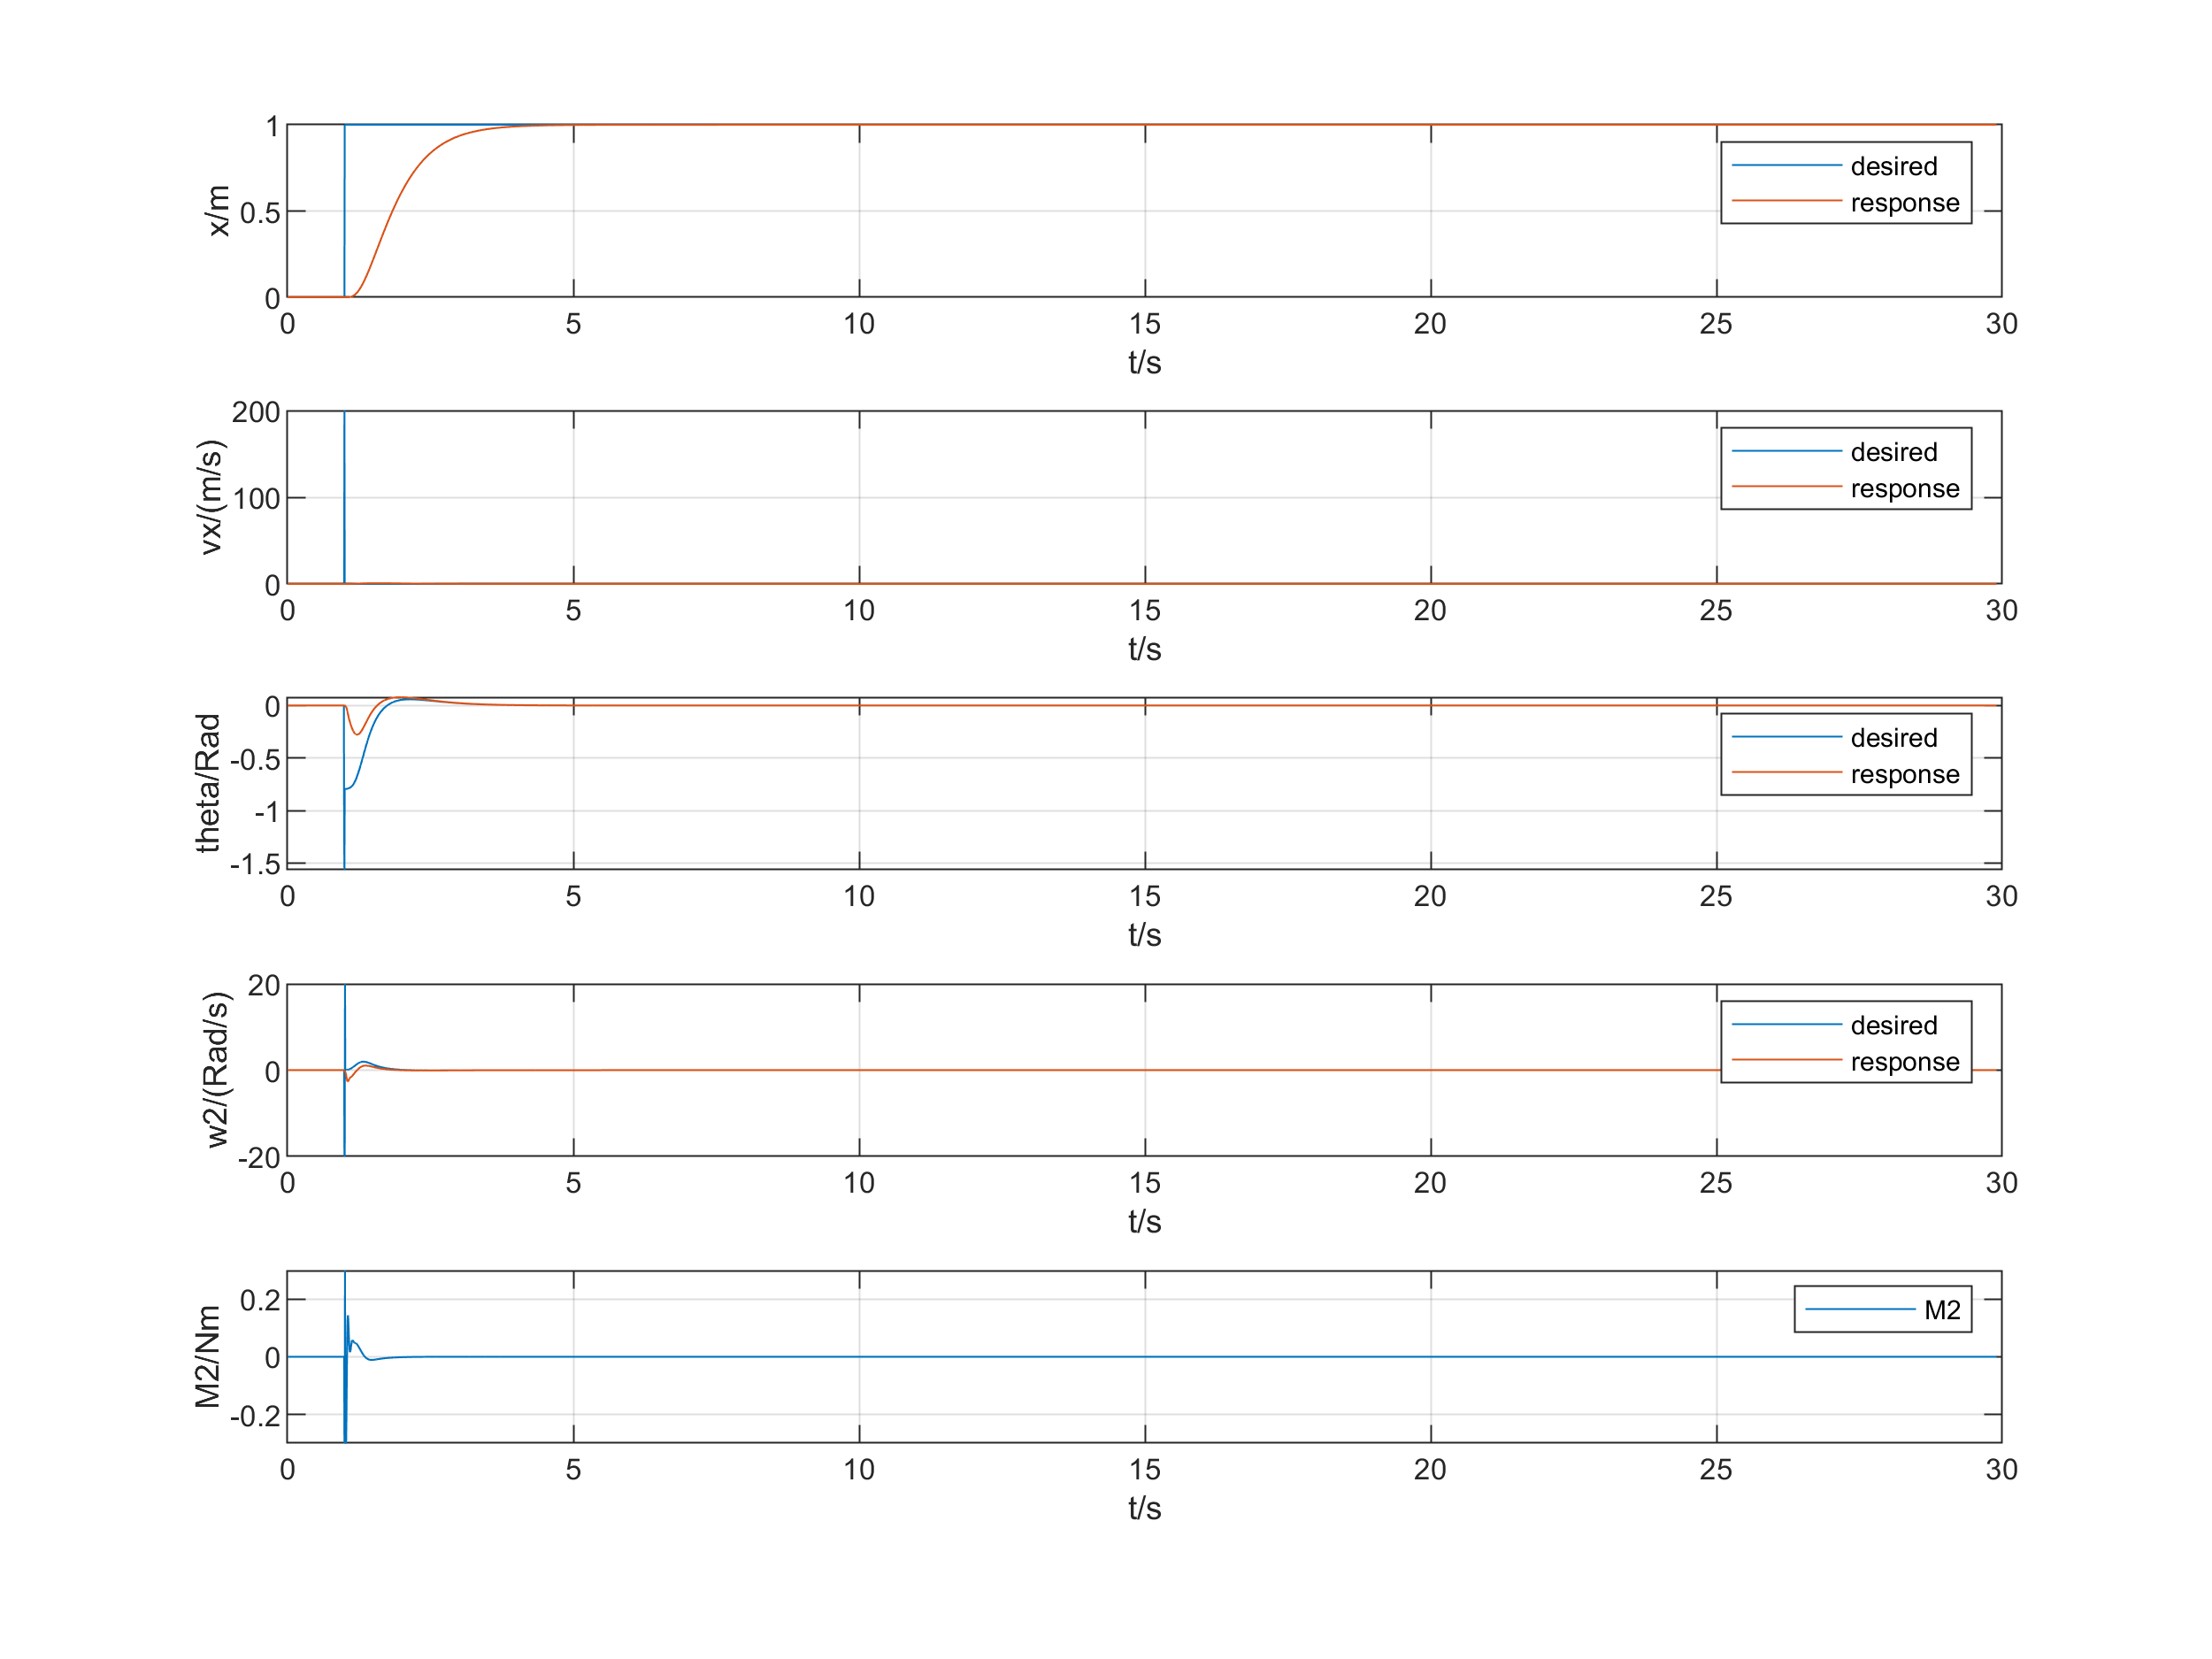
\includegraphics[width=\linewidth]{so3_1.png}
    \caption{SO(3)}
  \end{subfigure}
  \caption{x轴位置单位阶跃响应对比}
  \label{matlab_阶跃}
\end{figure}

位置的阶跃给速度的期望值带来了微分冲击,这个冲击进一步传导给期望俯仰角,导致期望转矩饱和,PX4在这种情况下出现了震荡。HOFA的扭矩饱和持续时间最小,并且对俯仰角的跟踪也是最好的。三种控制器最终都能无静差地收敛到单位值。定量比较三种控制器分别使位置到达稳态值$90\%$的上升时间和调整时间($\Delta = 5\%$):


\begin{table}[h]
  \centering
  \caption{单位阶跃响应性能对比}
  \begin{tabular}{cccc}
      \toprule
      & HOFA & PID & SO(3) \\
      \midrule
    上升时间 & 1.585s & 1.810s & 1.775s\\
    调整时间($\Delta = 5\%$) & 1.940s & 2.005s &2.145s \\
      \bottomrule
  \end{tabular}

  \label{matlab阶跃对比}
\end{table}
由表\ref{matlab阶跃对比}可知,HOFA的收敛速度要略微优于PID和SO(3)。

\textbf{单位斜坡输入}

接下来向x轴输入单位斜坡信号,对比x轴位置、速度、角度、角速度和期望扭矩,如图\ref{matlab_t}。

\begin{figure}[h]
  \centering
  \begin{subfigure}[t]{0.33\textwidth}
    \centering
    \raisebox{-\height}{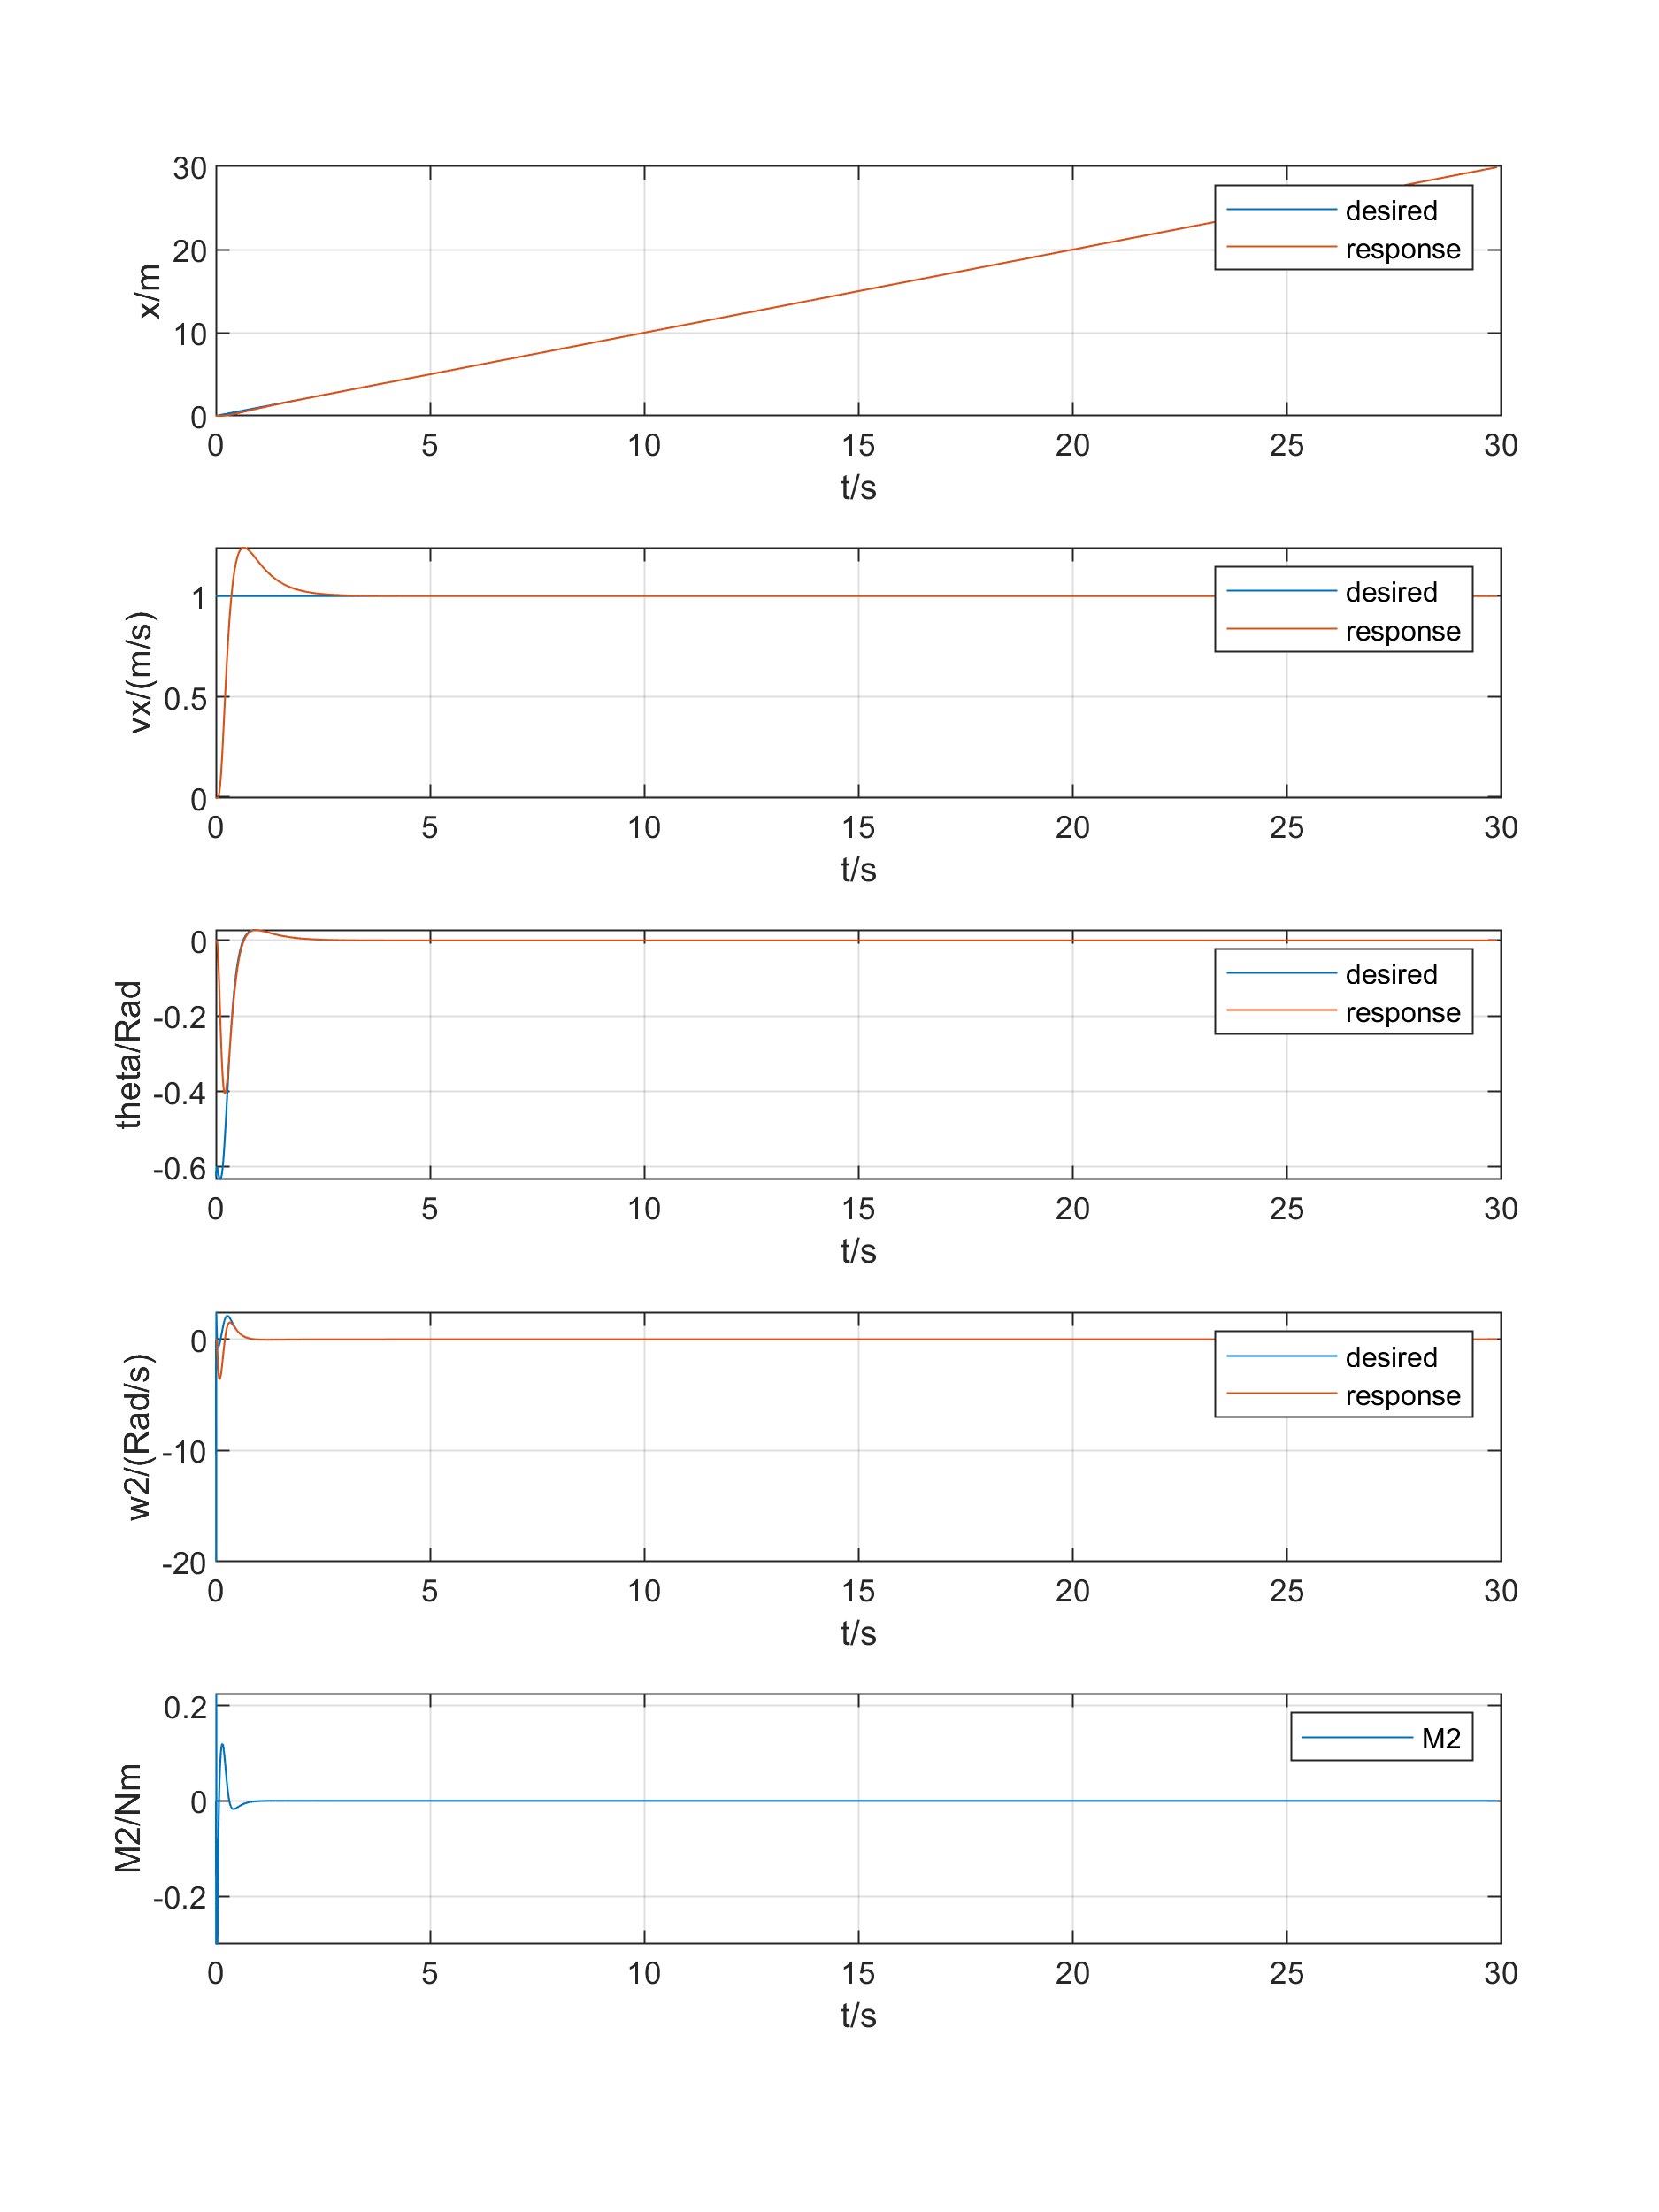
\includegraphics[width=\linewidth]{hofa_t.png}}
    \caption{HOFA}
  \end{subfigure}\hfill
  \begin{subfigure}[t]{0.33\textwidth}
    \centering
    \raisebox{-\height}{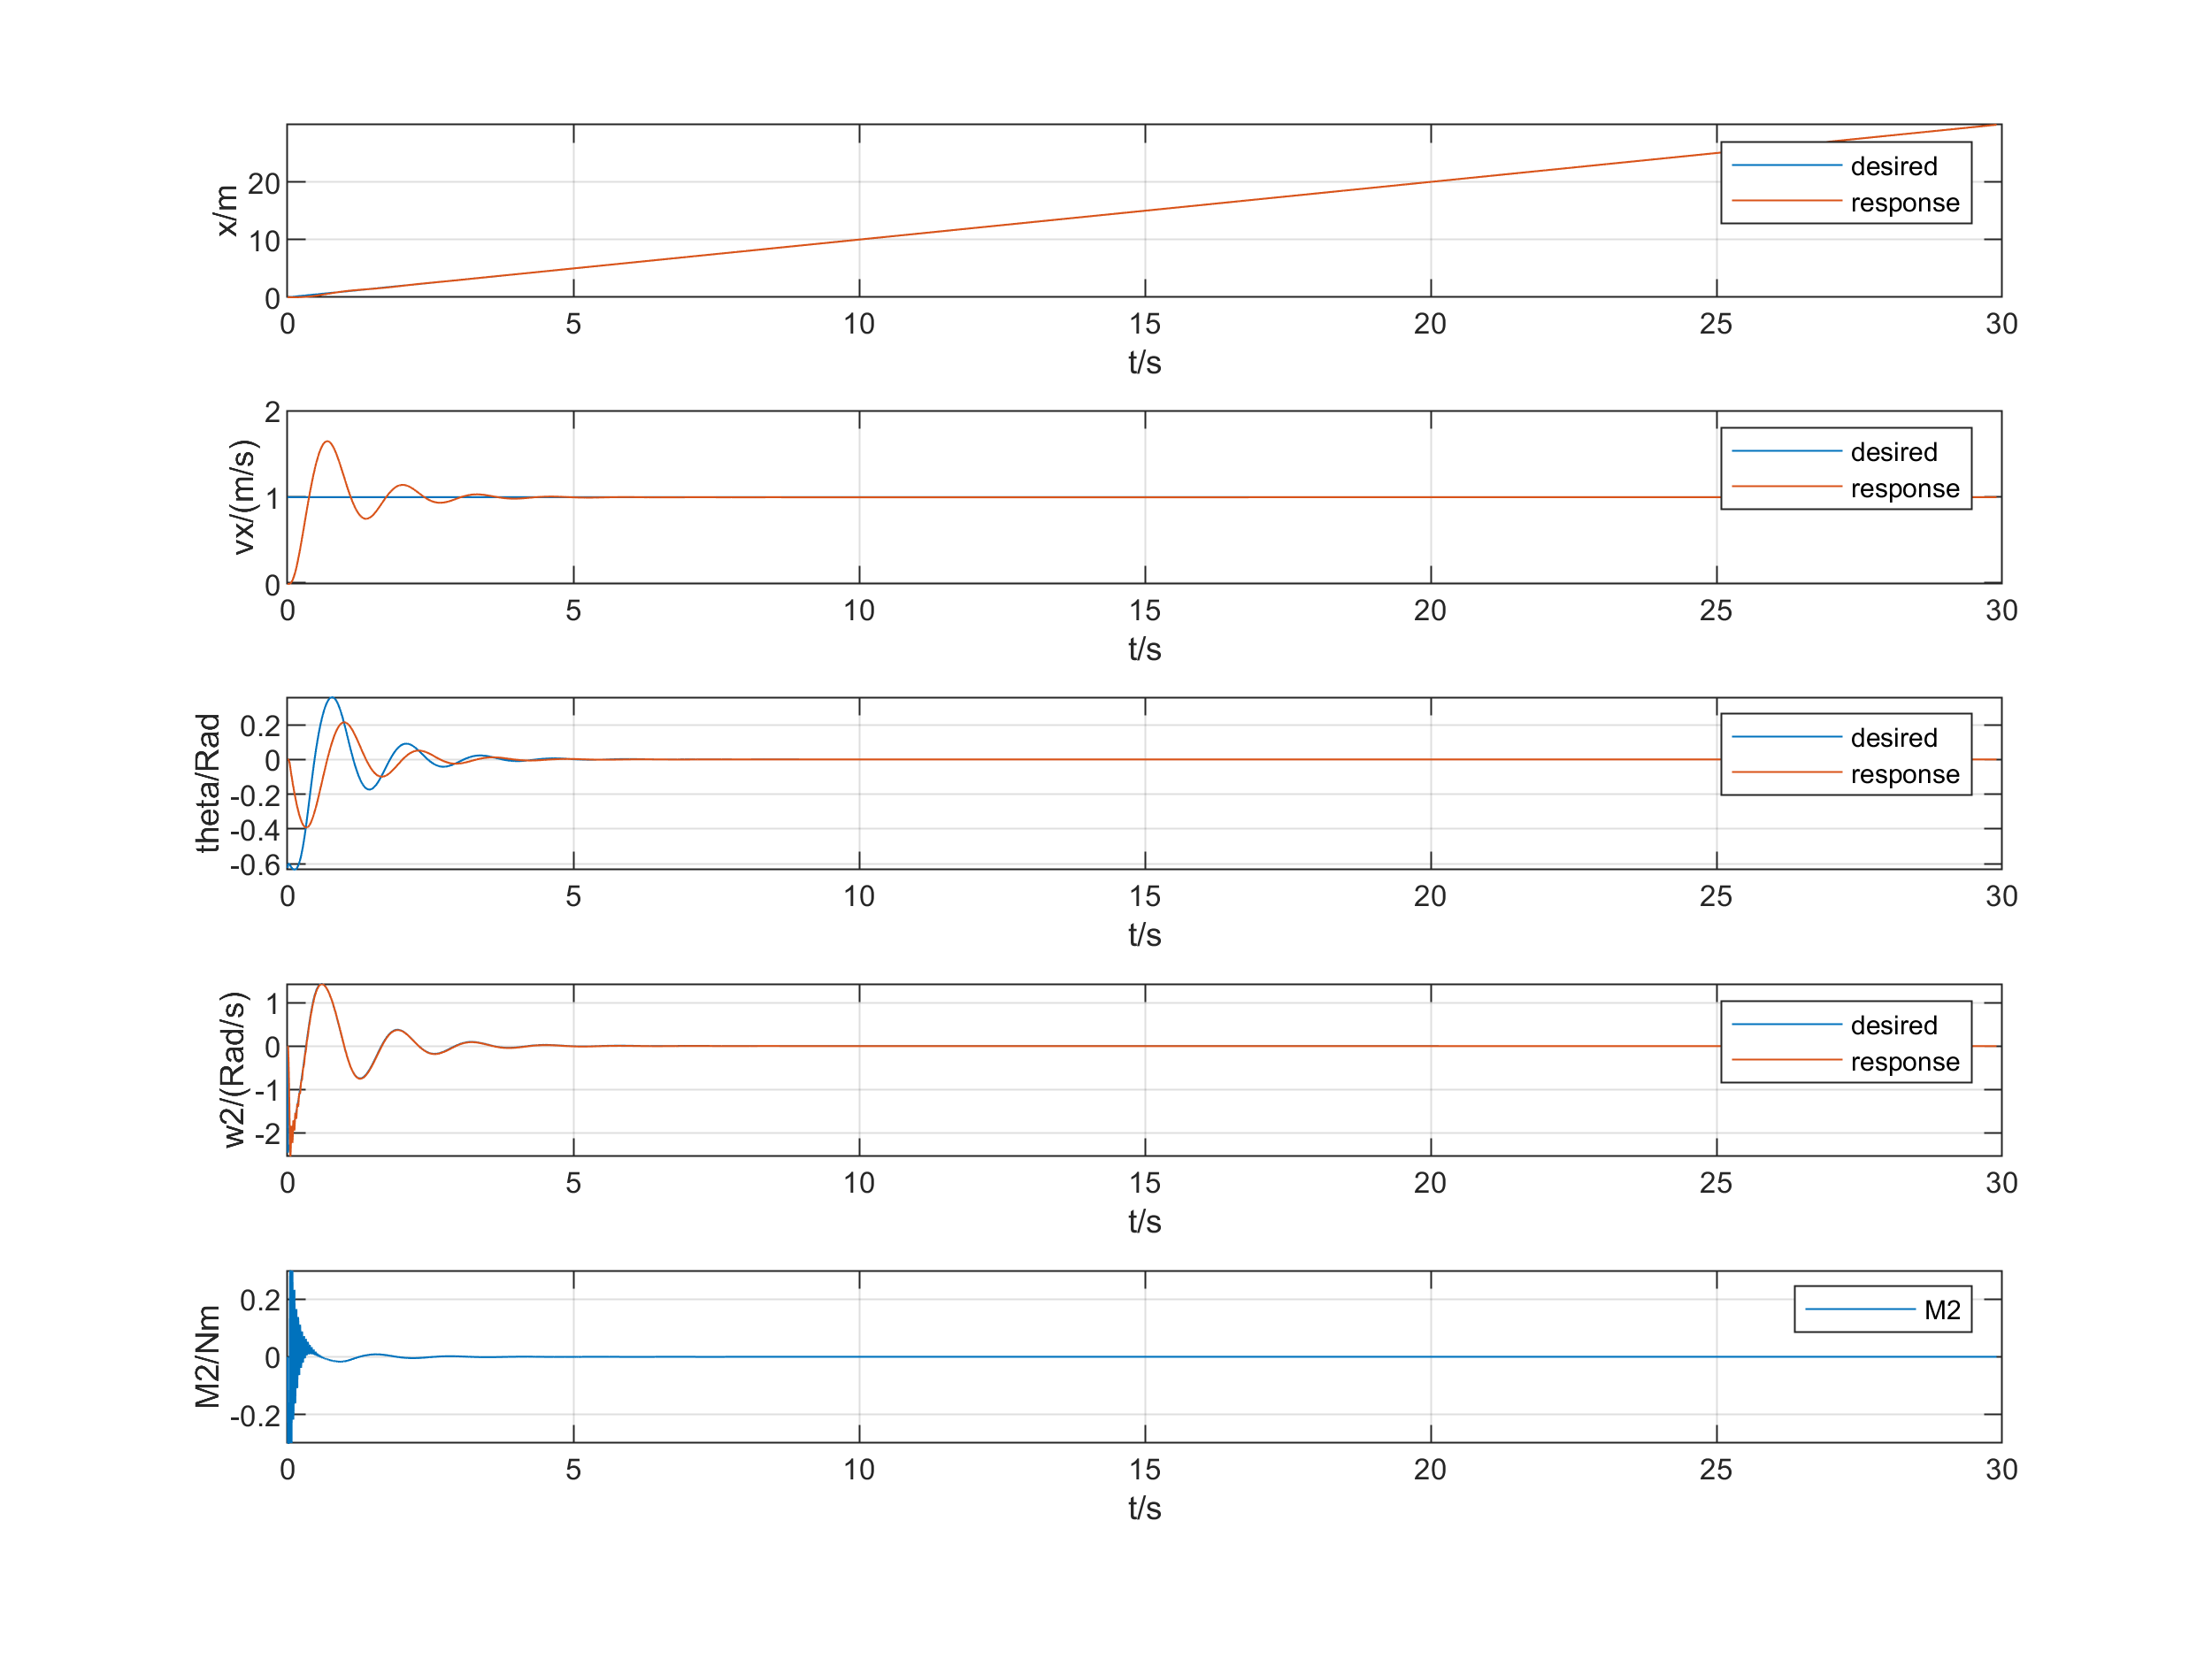
\includegraphics[width=\linewidth]{px4_t.png}}
    \caption{PID}
  \end{subfigure}\hfill
  \begin{subfigure}[t]{0.33\textwidth}
    \centering
    \raisebox{-\height}{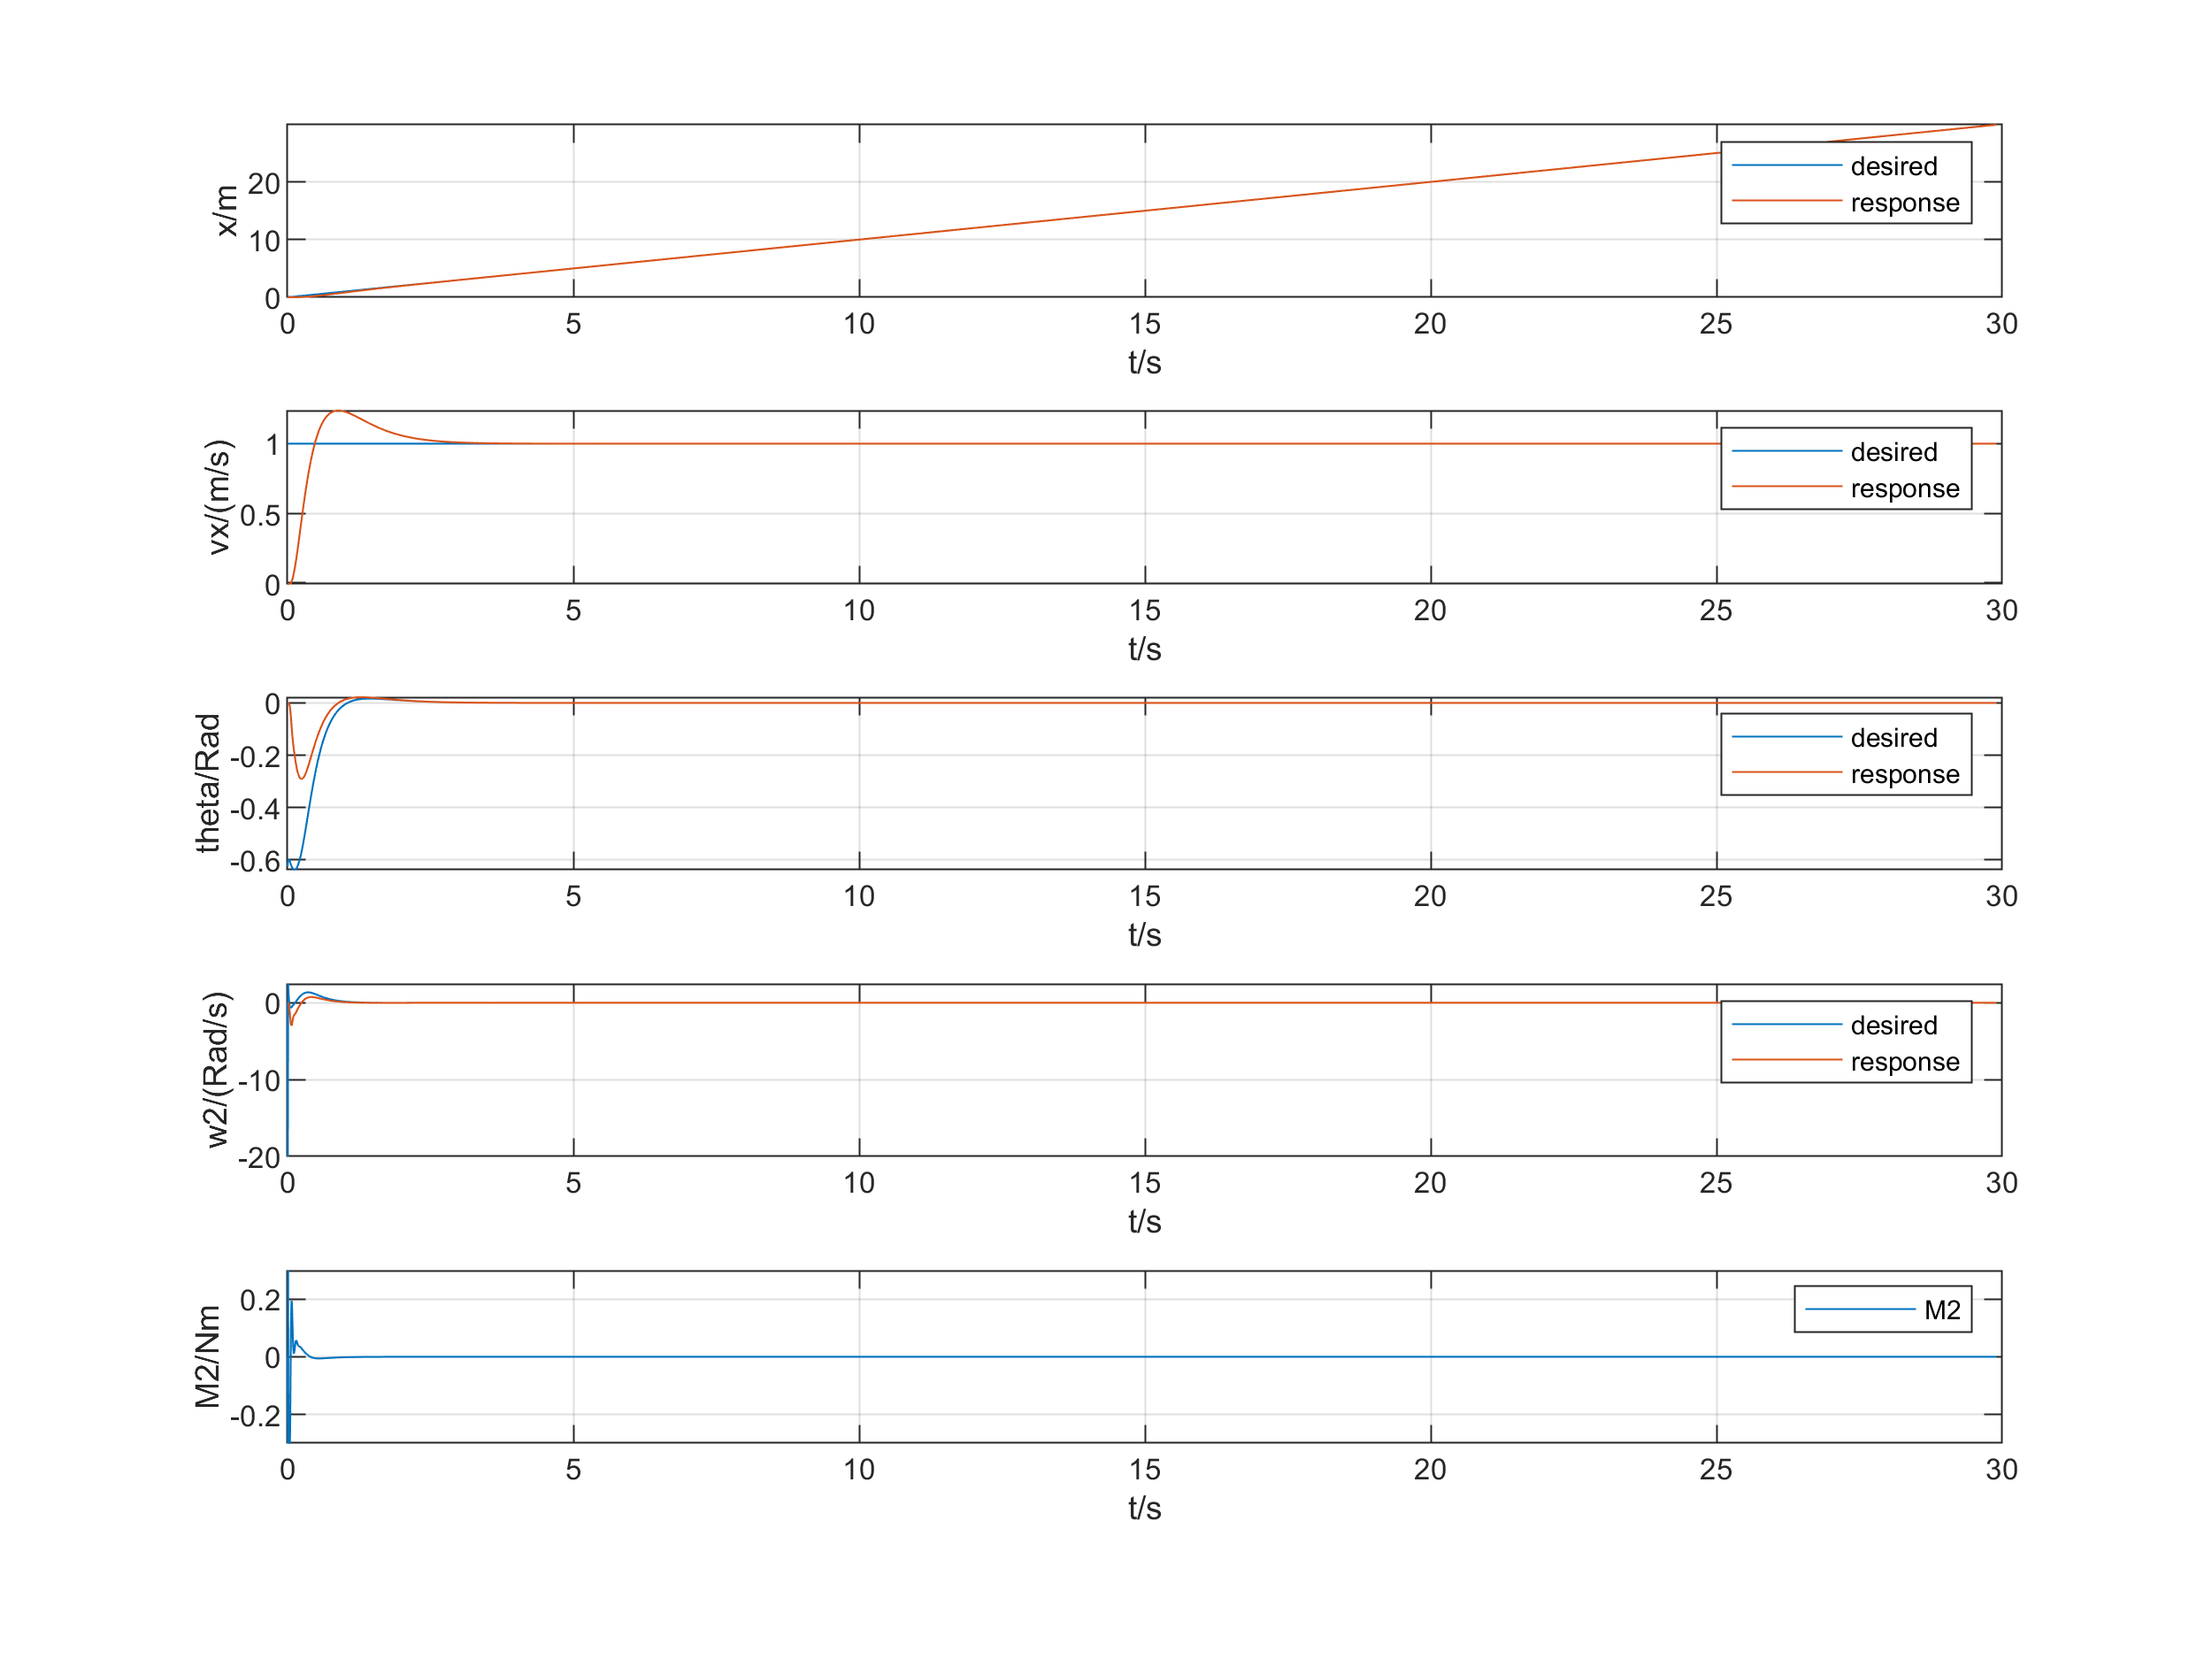
\includegraphics[width=\linewidth]{so3_t.png}}
    \caption{SO(3)}
  \end{subfigure}
  \caption{x轴位置单位斜坡响应对比}
  \label{matlab_t}
\end{figure}

位置的斜坡输入给速度和姿态角带来了阶跃输入,对于HOFA和SO(3)这两种依赖姿态微分来产生期望角速度的控制器,就使期望角速度和期望力矩饱和,而PID在这一环节只用了比例反馈就相对温和。在匀速飞行阶段,三者的姿态和角速度都保持稳定,这是仿真环境中没有噪声才能做到的。由于位置跟踪的静态误差都是0,因此进一步比较速度曲线,如表\ref{matlab斜坡对比}。三者的速度响应曲线都是欠阻尼,PID的波动更大,当然这可能是参数选择的问题,更快的响应速度意味着更大的超调,反之亦然。HOFA的上升时间小于其他两种控制器,超调量则略微大于SO(3)。调整时间是最优,说明HOFA的非线性前馈补偿项还是给动态过程带来了不小的优化。

\begin{table}[h]
  \centering
  \caption{单位斜坡响应性能对比}
  \begin{tabular}{cccc}
      \toprule
      & HOFA & PID & SO(3) \\
      \midrule
    位置静态误差                  & 0    & 0 & 0 \\
    速度上升时间                   & 0.37s & 0.385s &0.48s \\
    速度峰值时间                  & 0.66s &0.70s  & 0.90s\\
    速度最大超调量                & $32.0\%$ & $64.7\%$  & $23.7\%$\\
    速度调整时间($\Delta = 5\%$) & 1.67s &2.815s  & 2.09s\\
      \bottomrule
  \end{tabular}

  \label{matlab斜坡对比}
\end{table}

\textbf{综合测试}


  输入“8”字型轨迹测试控制器的综合性能,得到结果如图\ref{matlab_3d}。可以看出,三种控制方法都能较好地跟上期望轨迹,其中PID仅在开头处的偏差较大,HOFA和SO(3)在三维轨迹图中难以用肉眼分辨性能的高下。

  \newpage
  
  \begin{figure}[h]
      \centering
      \begin{subfigure}[t]{0.33\textwidth}
        \centering
        \raisebox{-\height}{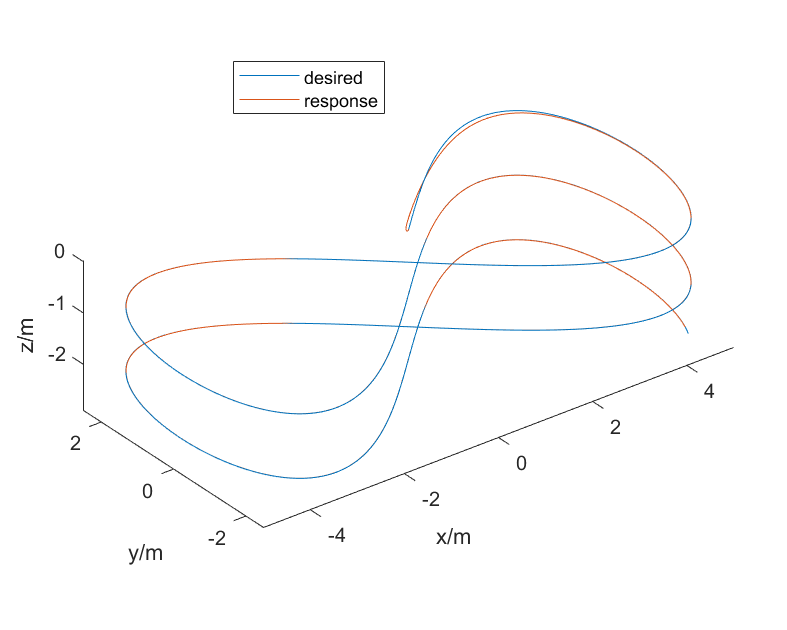
\includegraphics[width=\linewidth]{hofa_3d.png}}
        \caption{HOFA}
      \end{subfigure}\hfill
      \begin{subfigure}[t]{0.33\textwidth}
        \centering
        \raisebox{-\height}{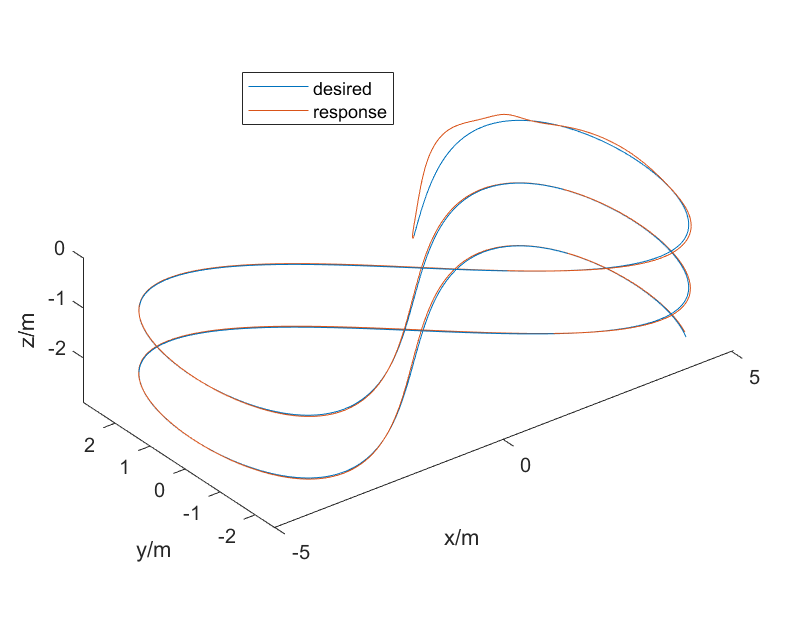
\includegraphics[width=\linewidth]{px4_3d.png}}
        \caption{PID}
      \end{subfigure}\hfill
      \begin{subfigure}[t]{0.33\textwidth}
        \centering
        \raisebox{-\height}{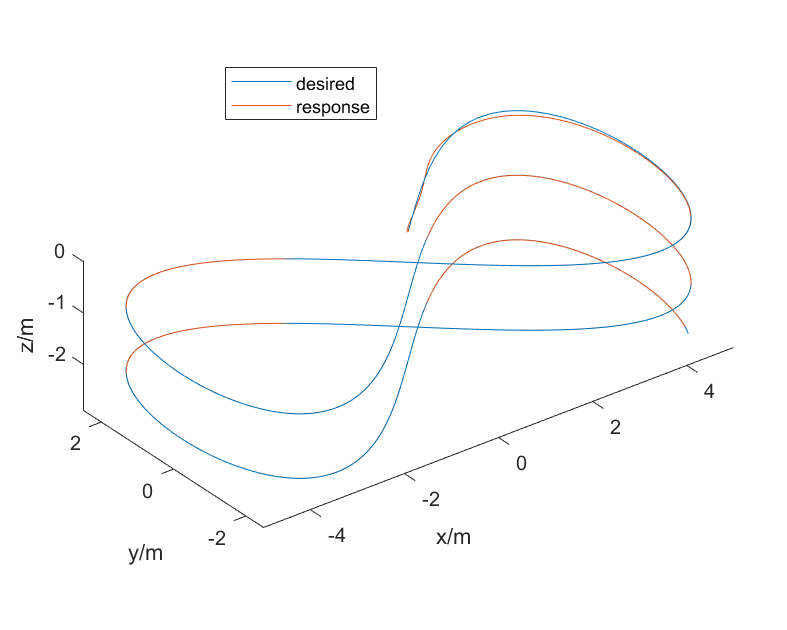
\includegraphics[width=\linewidth]{so3_3d.png}}
        \caption{SO(3)}
      \end{subfigure}
      \caption{三维轨迹跟踪效果对比}
      \label{matlab_3d}
  \end{figure}
 
  因此需要进一步看位置和姿态各轴分开的曲线:

  \begin{figure}[h]
    \centering
    \begin{subfigure}[t]{0.33\textwidth}
      \centering
      \raisebox{-\height}{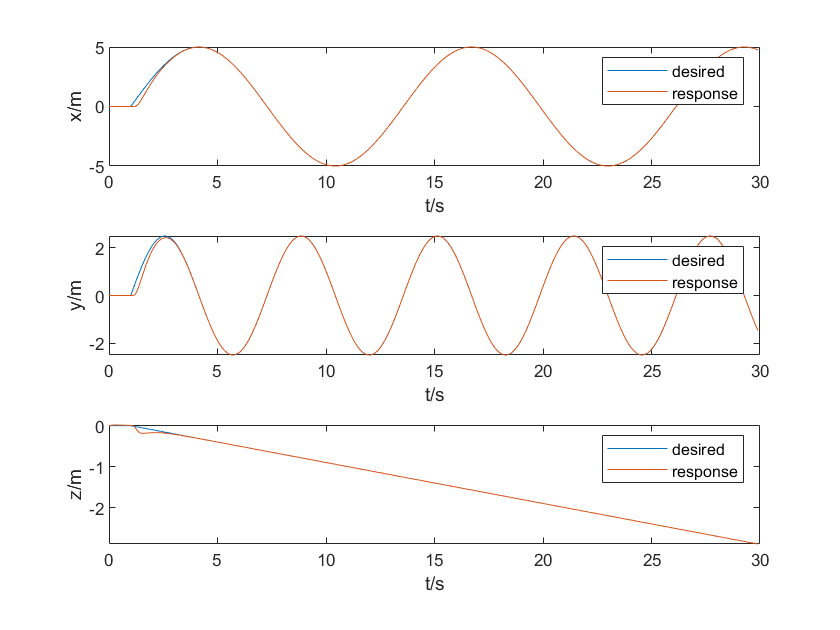
\includegraphics[width=\linewidth]{hofa_x.png}}
      \caption{HOFA}
    \end{subfigure}\hfill
    \begin{subfigure}[t]{0.33\textwidth}
      \centering
      \raisebox{-\height}{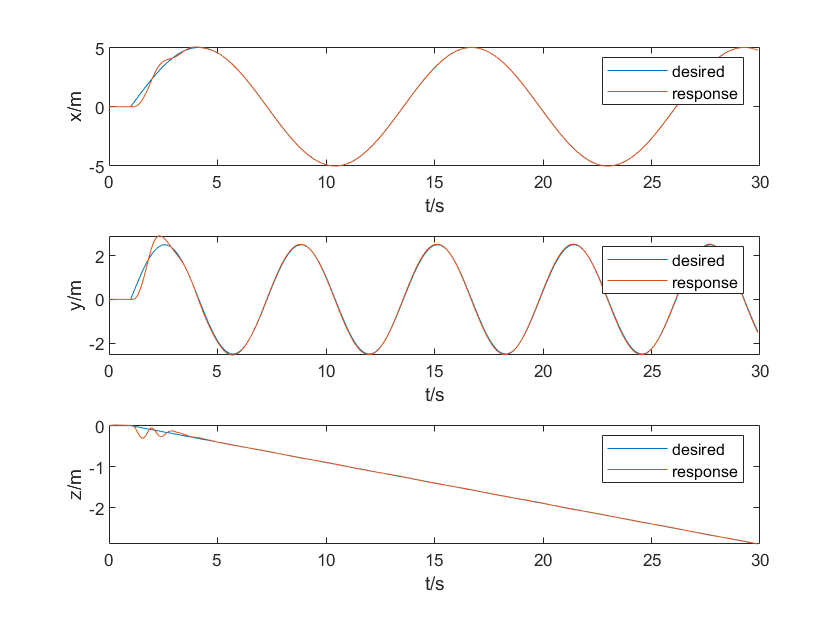
\includegraphics[width=\linewidth]{px4_x.png}}
      \caption{PID}
    \end{subfigure}\hfill
    \begin{subfigure}[t]{0.33\textwidth}
      \centering
      \raisebox{-\height}{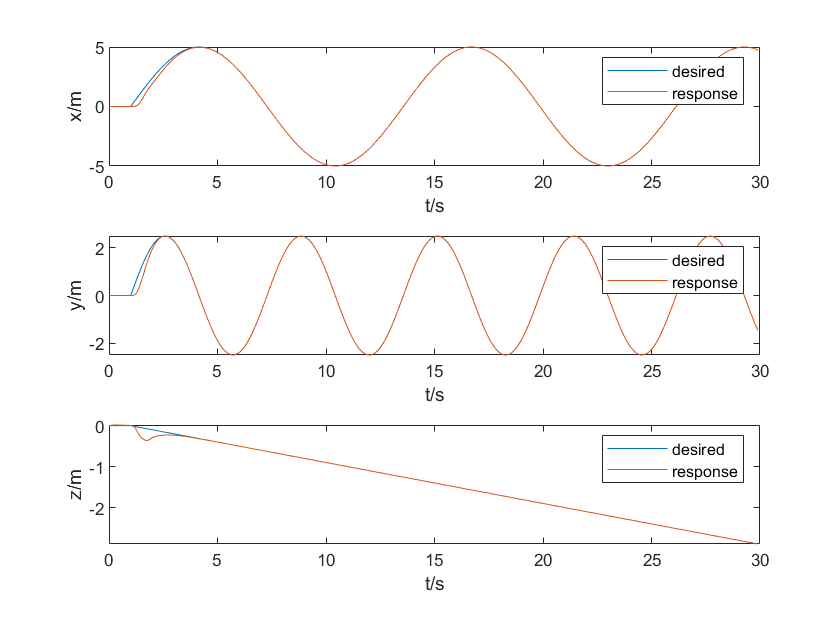
\includegraphics[width=\linewidth]{so3_x.png}}
      \caption{SO(3)}
    \end{subfigure}
    \caption{三轴位置跟踪效果对比}
    \label{matlab_x}
\end{figure}

\begin{figure}[h]
  \centering
  \begin{subfigure}[t]{0.33\textwidth}
    \centering
    \raisebox{-\height}{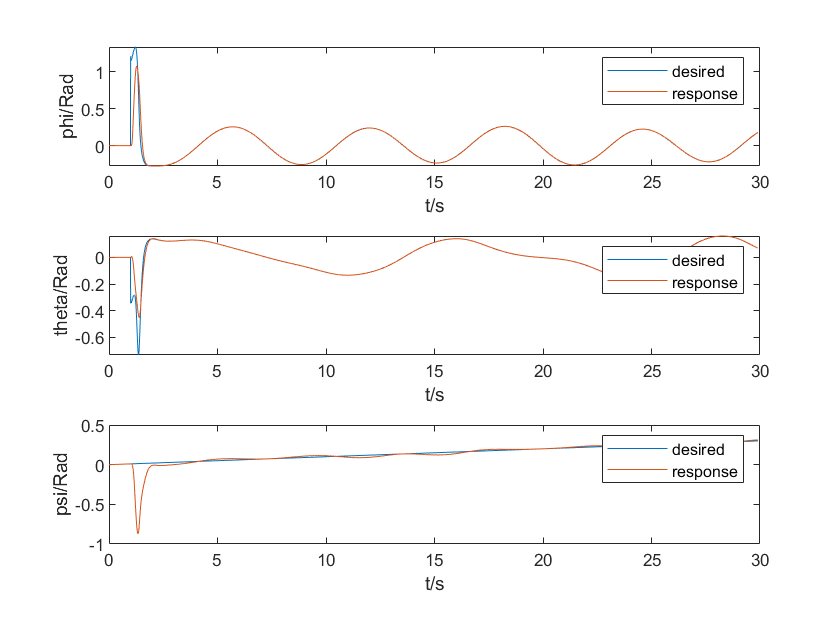
\includegraphics[width=\linewidth]{hofa_rad.png}}
    \caption{HOFA}
  \end{subfigure}\hfill
  \begin{subfigure}[t]{0.33\textwidth}
    \centering
    \raisebox{-\height}{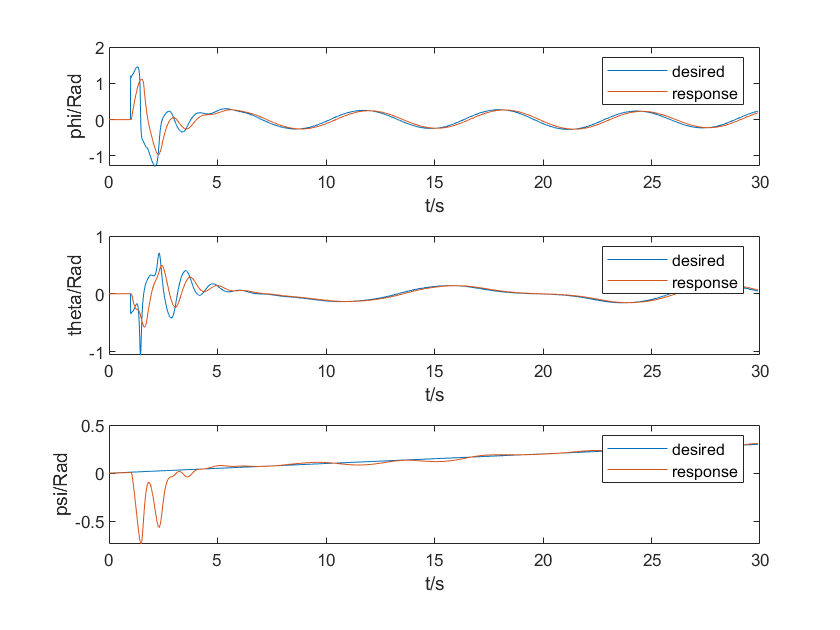
\includegraphics[width=\linewidth]{px4_angle.png}}
    \caption{PID}
  \end{subfigure}\hfill
  \begin{subfigure}[t]{0.33\textwidth}
    \centering
    \raisebox{-\height}{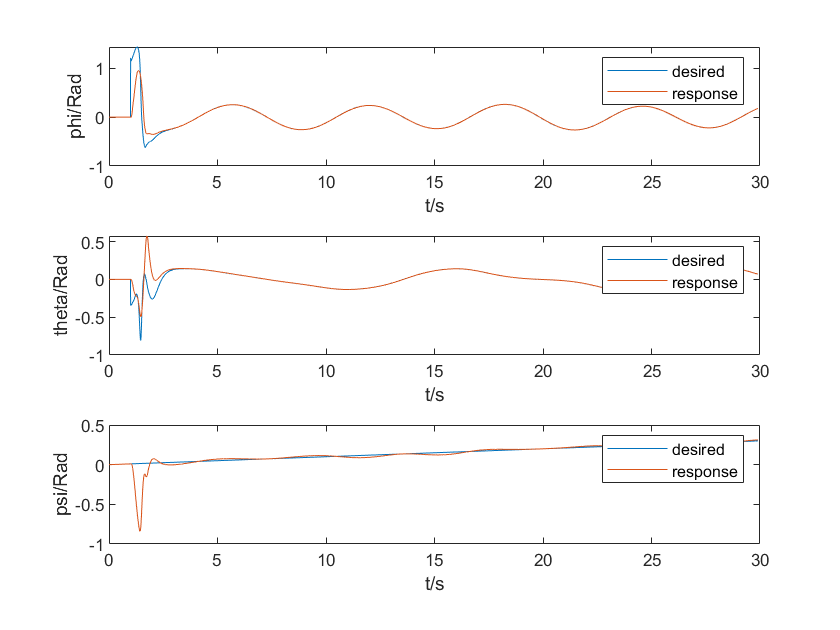
\includegraphics[width=\linewidth]{so3_angle.png}}
    \caption{SO(3)}
  \end{subfigure}
  \caption{三轴姿态角跟踪效果对比}
  \label{matlab_angle}
\end{figure}

从图\ref{matlab_x},\ref{matlab_angle}中来看,HOFA相较于SO(3)在位置环的优势并不明显,但在姿态环,HOFA的跟踪效果有较为显著的优势。在设定角度超过$50^\circ$的情况下,HOFA仍能做到良好的跟踪,同时保持飞机的稳定飞行。

  
为了定量地对比三者的跟踪性能,引入以下指标:
  $$e_d=\frac{\sum_0^{T}||x-x_d||}{T} \quad e_{angle}=\frac{\sum_0^{T}|\phi-\phi_d+\theta-\theta_d+\psi-\psi_d|}{T}$$

  $$J=\sum_0^{T}(p-p_d)^T Q_x(p-p_d)+u^T R_x u \quad p=\begin{bmatrix}
    x \\ v
  \end{bmatrix}$$
  \begin{table}[h]
    \centering
    \caption{HOFA方法与对照组的平均误差对比}
    \begin{tabular}{cccc}
        \toprule
        & 平均距离误差:$e_d$ (m)& 平均角度误差:$e_{angle}(Rad)$  & 最优控制指标:$J$ \\
        \midrule
        HOFA & 0.0296 & 0.0051 &49731 \\
        PID & 0.0710 & 0.0628 &54410 \\
        SO(3) &0.0408  &0.0143 &50277 \\
        \bottomrule
    \end{tabular}

    \label{matlab对比}
\end{table}

从表\ref{matlab对比}中可以看到,HOFA相较于PID和SO(3)均有不小的优势,尤其是在姿态控制上,HOFA能做到更高的跟踪精度。

在实践中,执行器的能力存在上限,并且轨迹中的不连续点会引起微分冲击,因此在控制器中必然要做限幅处理以避免极端大的控制量对系统造成不良影响。而限幅的具体数值也要根据控制器的输出做调整。从图\ref{matlab_fM}可知,除了在开头的阶跃处,当飞行进入稳定阶段时,期望的力矩非常小,远远不会达到设定的上限。
\begin{figure}[h]
  \centering
  \begin{subfigure}[t]{0.33\textwidth}
    \centering
    \raisebox{-\height}{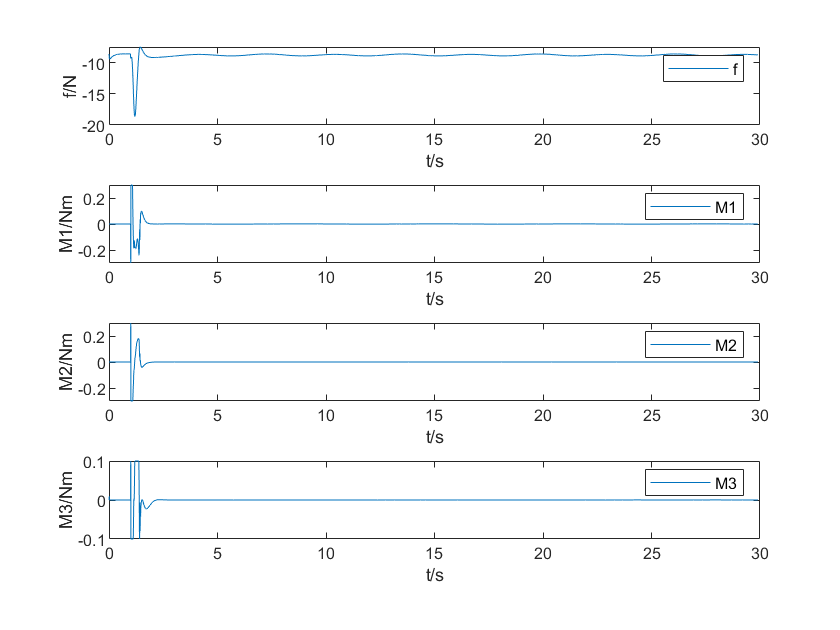
\includegraphics[width=\linewidth]{hofa_fM.png}}
    \caption{HOFA}
  \end{subfigure}\hfill
  \begin{subfigure}[t]{0.33\textwidth}
    \centering
    \raisebox{-\height}{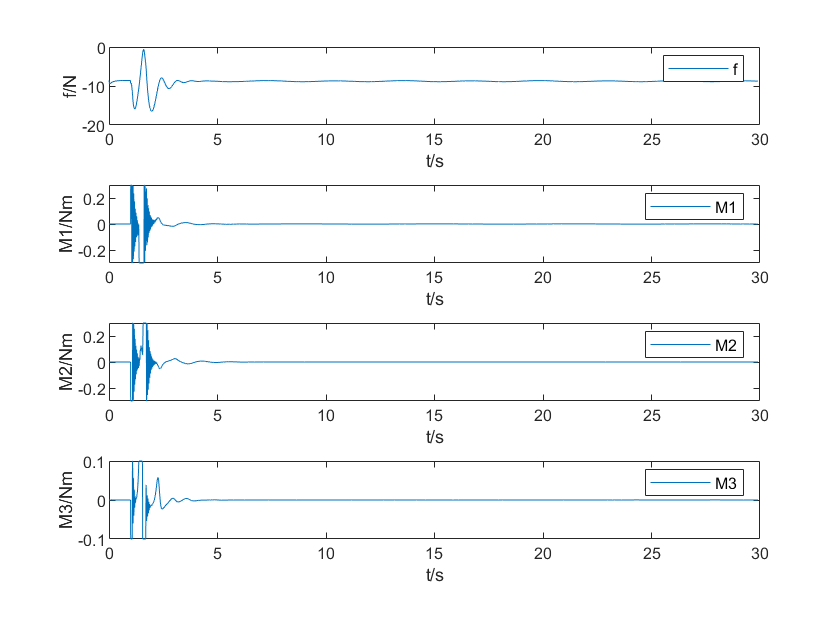
\includegraphics[width=\linewidth]{px4_fM.png}}
    \caption{PID}
  \end{subfigure}\hfill
  \begin{subfigure}[t]{0.33\textwidth}
    \centering
    \raisebox{-\height}{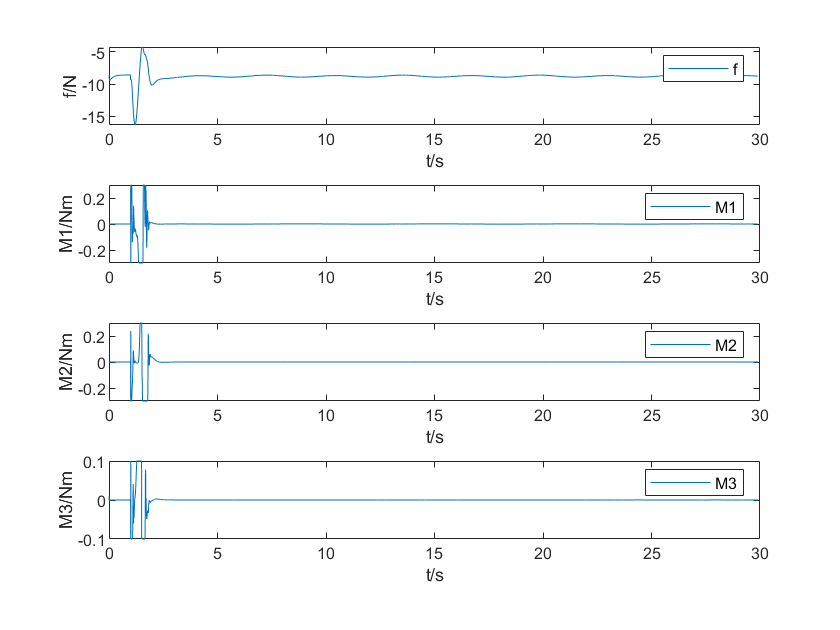
\includegraphics[width=\linewidth]{so3_fM.png}}
    \caption{SO(3)}
  \end{subfigure}
  \caption{期望拉力与力矩对比}
  \label{matlab_fM}
\end{figure}

% %%
% \begin{figure}[h]
%   \centering
%   \begin{subfigure}[t]{0.33\textwidth}
%     \centering
%     \raisebox{-\height}{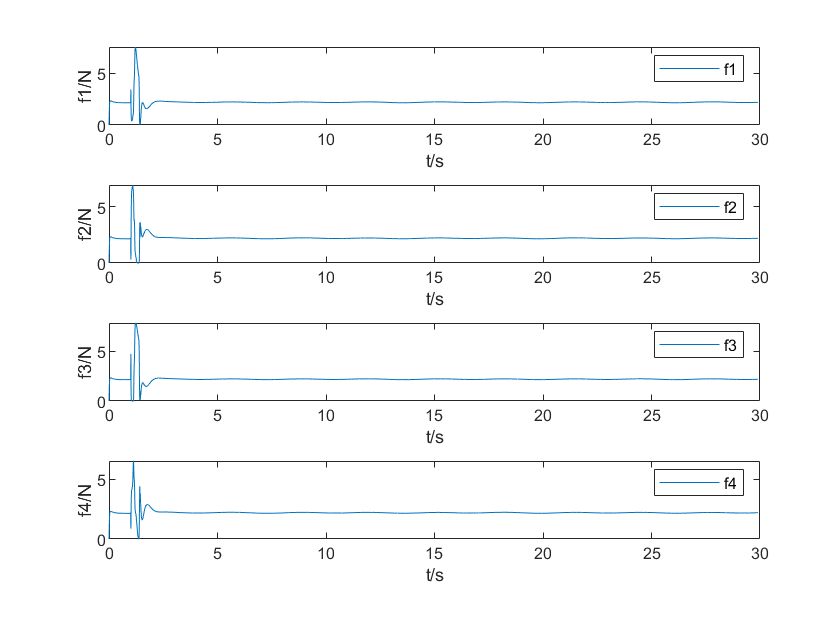
\includegraphics[width=\linewidth]{hofa_f1234.png}}
%   \end{subfigure}\hfill
%   \begin{subfigure}[t]{0.33\textwidth}
%     \centering
%     \raisebox{-\height}{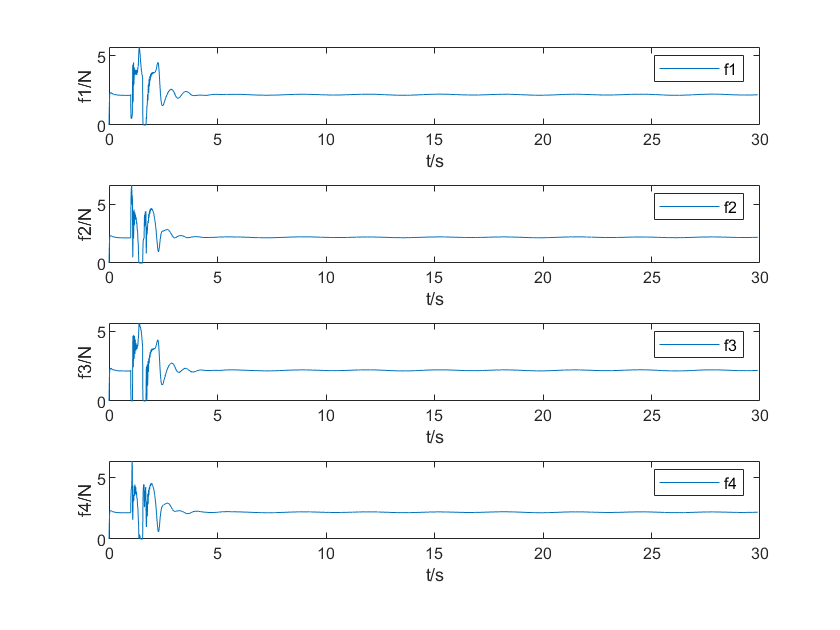
\includegraphics[width=\linewidth]{px4_f1234.png}}
%   \end{subfigure}\hfill
%   \begin{subfigure}[t]{0.33\textwidth}
%     \centering
%     \raisebox{-\height}{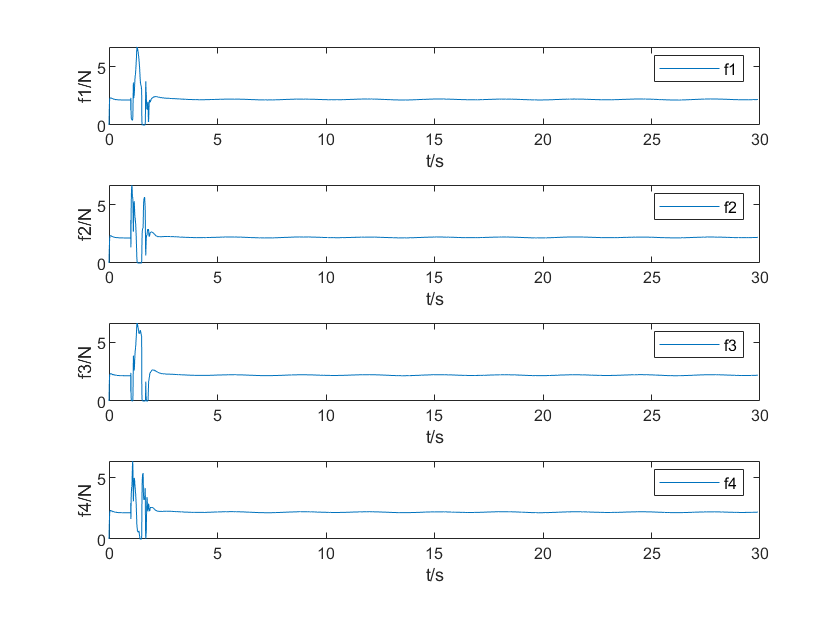
\includegraphics[width=\linewidth]{so3_f1234.png}}
%   \end{subfigure}
%   \caption{电机期望拉力对比:HOFA,PX4,SO(3)}
%   \label{matlab_f1234}
% \end{figure}

% %%
\section{力矩组分分析}
姿态环的输出的期望力矩由三部分组成,前两项可以视作前馈补偿,第三项可以视作反馈。除$wJw$外,都含有期望角速度,这会在外部输入出现不连续时带来冲击,$A_d$甚至含有期望角加速度,冲击更为剧烈。三部分均含有角速度,Matlab阶段较为理想,但在实机实验中角速度受电机振动影响,很容易出现高频的剧烈抖动,这也会带来不良影响,因此要降低角速度的反馈权重。
$$M=-B^{-1}(R_d,R) A_d(R_d,\omega_d,\dot \omega_d,R,\omega)+\omega \times J\omega +B^{-1}(R_d,R)M^*(R_d,\omega_d,R,\omega)$$

Matlab中虽然无法模拟角速度的高频抖动,但是能体现外部位置阶跃输入带来的期望角速度冲击给期望力矩计算带来的影响,如图\ref{fig:com}所示。在位置阶跃输入时,确实给$A_d$和$M^*$部分带来了冲击。在角速度很小的情况下,第二部分的数值几乎可以忽略。在大部分情况下,反馈项和整体的趋势相同,或者说反馈项主导了整体的走势。$A_d$和整体的吻合程度略低一些,$wJw$的走势则几乎与整体无关。

\begin{figure}[!h]
  \centering
  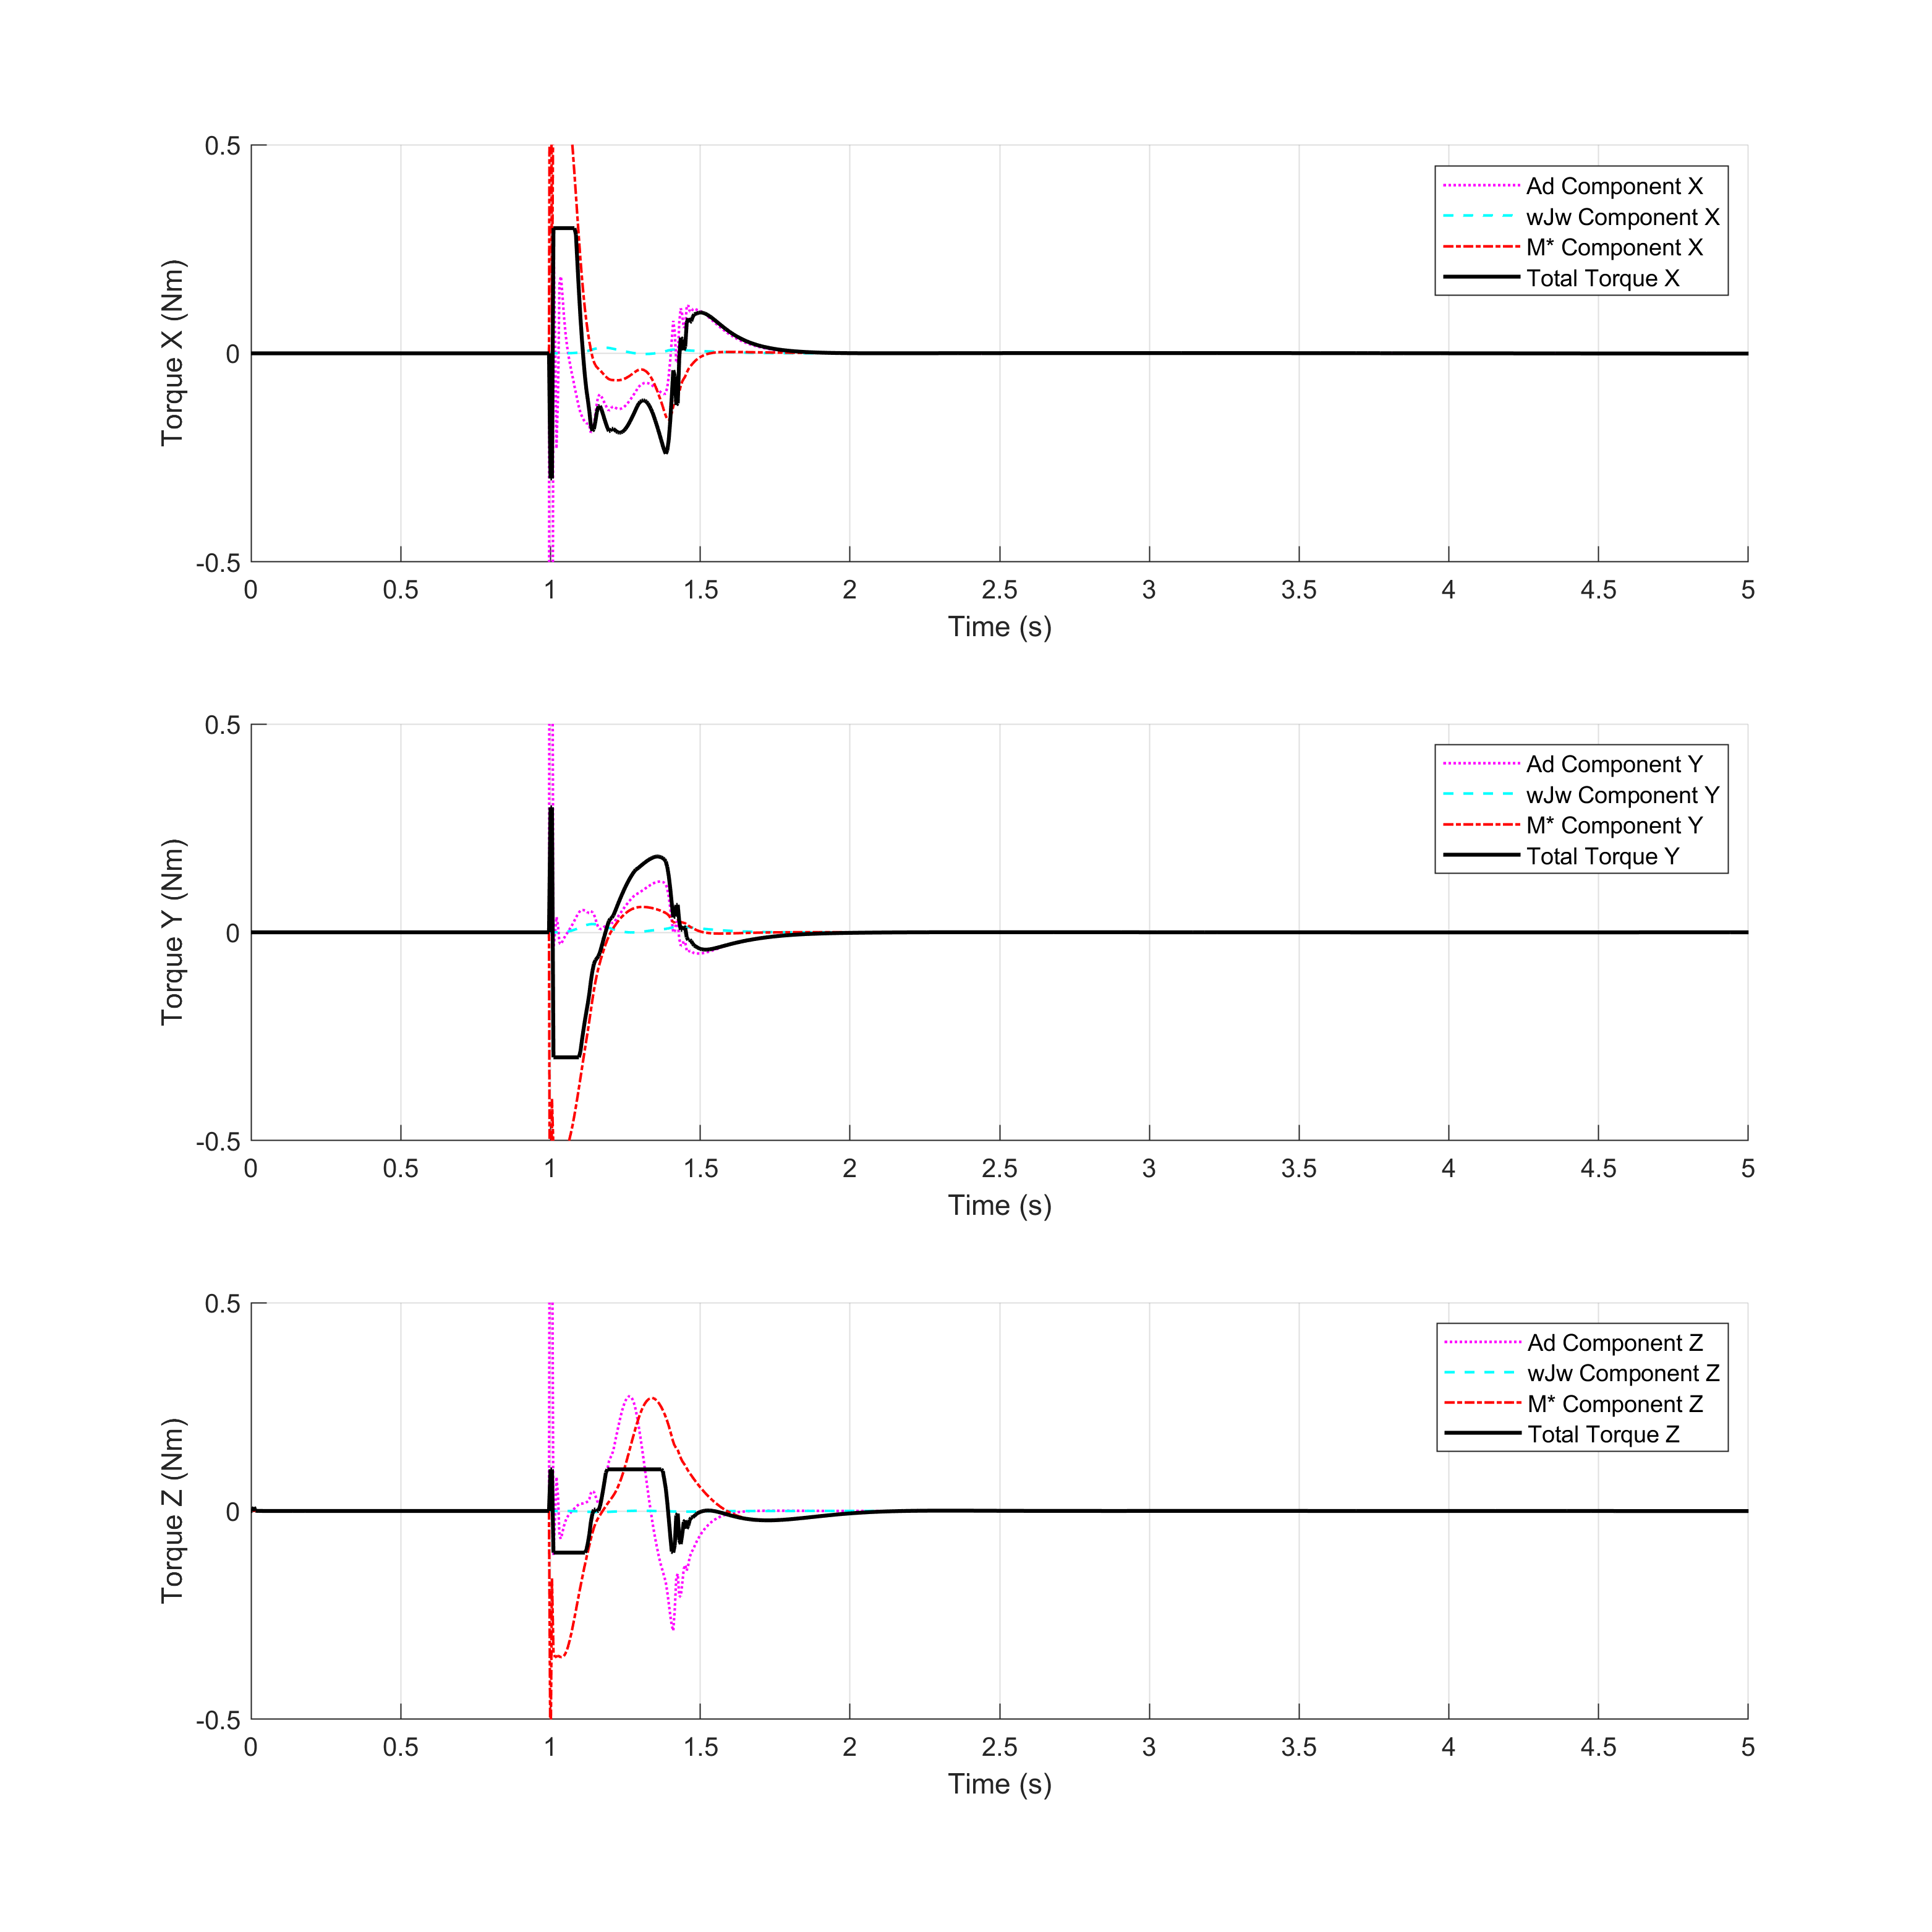
\includegraphics[width=0.65\textwidth]{component.png}
  \caption{姿态环输出期望力矩组成}
  \label{fig:com}
\end{figure}

\section{本章小结}
本章介绍了在Matlab中的实验设计,将HOFA与经典的控制方法对比并根据实验数据展开分析。在单位阶跃和单位斜坡信号的输入下,HOFA具有更快的收敛速度和追踪性能。在“8”字型轨迹的综合测试下,HOFA具有更高的跟踪精度,并且在优化指标上,验证了LQR的最优性能。总而言之,在较为接近理想化模型的Matlab仿真中,HOFA展现出了相较于PID和SO(3)两种经典控制方法的优势。